\chapter{The Simulation Library}
\label{cha:the-simulation-library}

{\opp} has an extensive C++ class library available to the user for
implementing simulation models and model components. Part of the class
library's functionality has already been covered in the previous chapters,
including discrete event simulation basics, the simple module programming
model, module parameters and gates, scheduling events, sending and
receiving messages, channel operation and programming model, finite state
machines, dynamic module creation, signals, and more.

This chapter discusses the rest of the simulation library. Topics will
include logging, random number generation, queues, topology discovery and
routing support, and statistics and result collection. This chapter also
covers some of the conventions and internal mechanisms of the simulation
library to allow one extending it and using it to its full potential.


\section{Fundamentals}

\subsection{Using the Library}
\label{sec:ch-sim-lib:using-omnetpp}

Classes in the {\opp} simulation library are part of the \ttt{omnetpp}
namespace. To use the {\opp} API, you must include the \ttt{omnetpp.h}
header file and either import the namespace with \ttt{using namespace
omnetpp}, or qualify names with the \ttt{omnetpp::} prefix.

\subsection{The cObject Base Class}
\label{sec:ch-sim-lib:cobject}

Most classes in the simulation library are derived from \cclass{cObject},
or its subclasses \cclass{cNamedObject} and \cclass {cOwnedObject}.
\cclass{cObject} defines several virtual member functions that are either
inherited or redefined by subclasses. Otherwise, \cclass{cObject} is a
zero-overhead class as far as memory consumption goes: it purely defines an
interface but has no data members. Thus, having \cclass{cObject} a base
class does not add anything to the size of a class if it already has at
least one virtual member function.

\begin{figure}[htbp]
 \begin{center}
   \includegraphics[height=6cm]{figures/cobject-inheritance}
   \caption{cObject is the base class for most of the simulation library}
  \end{center}
\end{figure}

The subclasses \cclass{cNamedObject} and \cclass {cOwnedObject} add data
members to implement more functionality. The following sections discuss
some of the practically important functonality defined by \cclass{cObject}.


\subsubsection{Name and Full Name}
\label{sec:sim-lib:name}
\index{object!name}

The most useful and most visible member functions of \cclass{cObject} are
\ffunc{getName()} and \ffunc{getFullName()}. The idea behind them is that
many objects in {\opp} have names by default (for example, modules,
parameters and gates), and even for other objects, having a printable name
is a huge gain when it comes to logging and debugging.

\ffunc{getFullName()} is important for gates and modules, which may be part
of gate or module vectors. For them, \ffunc{getFullName()} returns the name
with the index in brackets, while \ffunc{getName()} only returns the name
of the module or gate vector. That is, for a gate \ttt{out[3]} in the gate
vector \ttt{out[10]}, \ffunc{getName()} returns \ttt{"out"}, and
\ffunc{getFullName()} returns \ttt{"out[3]"}. For other objects,
\ffunc{getFullName()} simply returns the same string as \ffunc{getName()}.
An example:

\begin{cpp}
cGate *gate = gate("out", 3);  // out[3]
EV << gate->getName();  // prints "out"
EV << gate->getFullName();  // prints "out[3]"
\end{cpp}

\begin{note}
If you don't know the runtime type of an object, prefer \ffunc{getFullName()}
when printing its name, so you don't miss out the index if the object has one.
\end{note}

\cclass{cObject} merely defines these member functions, but they return an
empty string. Actual storage for a name string is provided by the class
\cclass{cNamedObject}, which also has a \ffunc{setName()} method. Since
most library classes are derived from \cclass{cNamedObject}, you can assign
arbitrary names to objects if {\opp} does not already provides them with
one.

By convention, the object name is the first argument to the constructor
of every class, and it defaults to the empty string. To create an object with
a name, pass the name string (a \ttt{const char*} pointer) as the first
argument of the constructor. For example:

\begin{cpp}
cMessage *timeoutMsg = new cMessage("timeout");
\end{cpp}

To change the name of an object, use \cclass{setName()}:

\begin{cpp}
timeoutMsg->setName("timeout");
\end{cpp}

Both the constructor and \ffunc{setName()} make an internal copy of the string,
instead of just storing the pointer passed to them.\footnote{
  In a simulation, there are usually many objects with the same name:
  modules, parameters, gates, etc. To conserve memory, several classes
  keep names in a shared, reference-counted \textit{name pool} instead of
  making separate copies for each object. The runtime cost of looking up an
  existing string in the name pool and incrementing its reference count
  also compares favorably to the cost of allocation and copying.}

For convenience and efficiency reasons, the empty string \ttt{""}
and \ttt{nullptr} are treated as interchangeable by library objects.
That is, \ttt{""} is stored as \ttt{nullptr} but returned as \ttt{""}.
If you create a message object with either \ttt{nullptr}
or \ttt{""} as its name string, it will be stored as \ttt{nullptr}
and \ffunc{getName()} will return a pointer to a static \ttt{""}.


\subsubsection{Hierarchical Name}
\label{sec:sim-lib:fullpath}
\index{object!fullpath}

\ffunc{getFullPath()} returns the object's hierarchical name. This name is
produced by prepending the \textit{full name} (\ffunc{getFullName()}) with
the parent or owner object's \ffunc{getFullPath()}, separated by a dot. For
example, if the \ttt{out[3]} gate in the previous example belongs to a
module named \ttt{classifier}, which in turn is part of a network called
\ttt{Queueing}, then the gate's \ffunc{getFullPath()} method will return
\ttt{"Queueing.classifier.out[3]"}.

\begin{cpp}
cGate *gate = gate("out", 3);  // out[3]
EV << gate->getName();  // prints "out"
EV << gate->getFullName();  // prints "out[3]"
EV << gate->getFullPath();  // prints "Queueing.classifier.out[3]"
\end{cpp}

The \ffunc{getFullName()} and \ffunc{getFullPath()} methods are
extensively used in graphical runtime environments (Tkenv, Qtenv),
and also when assembling runtime error messages.

In contrast to \ffunc{getName()} and \ffunc{getFullName()} which return
\ttt{const char *} pointers, \ffunc{getFullPath()} returns
\ttt{std::string}. This makes no difference when logging via \ttt{EV<<},
but when \ffunc{getFullPath()} is used as a \ttt{"\%s"} argument to
\ffunc{sprintf()} you have to write \ttt{getFullPath().c\_str()}.

\begin{cpp}
char buf[100];
sprintf("msg is '%80s'", msg->getFullPath().c_str()); // note c_str()
\end{cpp}


\subsubsection{Class Name}
\label{sec:sim-lib:classname}

The \ffunc{getClassName()} member function returns the class
name as a string, including the namespace. \ffunc{getClassName()} internally
relies on C++ RTTI.

An example:

\begin{cpp}
const char *className = msg->getClassName(); // returns "omnetpp::cMessage"
\end{cpp}

%% \subsubsection{Owner}
%% \label{sec:sim-lib:owner}
%%
%% TODO

\subsubsection{Cloning Objects}
\label{sec:sim-lib:dup}

The \ffunc{dup()} member function creates an exact copy of the
object\index{object!copy}, duplicating\index{object!duplication}
contained objects also if necessary. This is especially useful in the
case of message objects.

\begin{cpp}
cMessage *copy = msg->dup();
\end{cpp}

\ffunc{dup()} delegates to the copy constructor. Classes also declare
an assignment operator (\ffunc{operator=()}) which can be used to copy contents
of an object into another object of the same type. \ffunc{dup()}, the copy
constructor and the assignment operator all perform deep coping: objects
contained in the copied object will also be duplicated if necessary.

\ffunc{operator=()} differs from the other two in that it does \textit{not}
copy the object's name string, i.e. does not invoke \ffunc{setName()}.
The rationale is that the name string is often used for identifying the particular
object instance, as opposed to being considered as part of its contents.

%% \subsubsection{Foreach}
%% \label{sec:sim-lib:foreach}
%%
%% TODO

\subsection{Iterators}

There are several container classes in the library (\cclass{cQueue},
\cclass{cArray} etc.) For many of them, there is a corresponding
iterator class that you can use to loop through the objects stored in
the container.

For example:

\begin{cpp}
cQueue queue;

//...
for (cQueue::Iterator it(queue); !it.end(); ++it) {
    cObject *containedObject = *it;
    //...
}
\end{cpp}

\subsection{Runtime Errors}

When library objects detect an error condition, they throw a C++ exception.
This exception is then caught by the simulation environment which pops up
an error dialog or displays the error message.

At times it can be useful to be able stop the simulation at the place of
the error (just before the exception is thrown) and use a C++ debugger to
look at the stack trace and examine variables. Enabling the
\fconfig{debug-on-errors} or the \fconfig{debugger-attach-on-error}
configuration option lets you do that -- check it in section
\ref{sec:ch-run-sim:controlling}.


\section{Logging from Modules}

In a simulation there are often thousands of modules which simultaneously carry
out non-trivial tasks. In order to understand a complex simulation, it is
essential to know the inputs and outputs of algorithms, the information on
which decisions are based, and the performed actions along with their parameters.
In general, logging facilitates understanding which module is doing what and why.

{\opp} makes logging easy and consistent among simulation models by providing
its own C++ API and configuration options. The API provides efficient logging
with several predefined log levels, global compile time and runtime filters,
per-component runtime filters, automatic context information, log prefixes and
other useful features. In the following sections, we look at how to write log
statements using the {\opp} logging API.

\subsection{Log Output}

The exact way log messages are displayed to the user depends on the user interface.
In the command-line user interface (Cmdenv\index{Cmdenv}), the log is simply
written to the standard output. In the graphical user interfaces, Tkenv and Qtenv,
the main window displays the log output of all modules by default. You can also
open new output windows on a per module basis, these windows automatically filter
for the log messages of the selected module.

\subsection{Log Levels}

All logging must be categorized into one of the predefined log levels. The
assigned log level determines how important and how detailed a log statement
is. When deciding which log level is appropriate for a particular log statement,
keep in mind that they are meant to be local to components. There's no need for
a global agreement among all components, because {\opp} provides per component
filtering. Log levels are mainly useful because log output can be filtered
based on them.

\begin{itemize}
  \item \fmac{LOGLEVEL\_OFF} is not a real log level, it can't be used for actual
    logging. It is only useful for configuration purposes, it completely disables
    logging.
  \item \fmac{LOGLEVEL\_FATAL} is the highest log level. It should be used for
    fatal (unrecoverable) errors that prevent the component from further
    operation. It doesn't mean that the simulation must stop immediately
    (because in such cases the code should throw a cRuntimeError), but rather
    that the a component is unable to continue normal operation. For example, a
    special purpose recording component may be unable to continue recording due
    to the disk being full.
  \item \fmac{LOGLEVEL\_ERROR} should be used for recoverable (non-fatal)
    errors that allow the component to continue normal operation. For example,
    a MAC layer protocol component could log unsuccessful packet receptions and
    unsuccessful packet transmissions using this level.
  \item \fmac{LOGLEVEL\_WARN} should be used for exceptional (non-error)
    situations that may be important for users and rarely occur in the
    component. For example, a MAC layer protocol component could log detected
    bit errors using this level.
  \item \fmac{LOGLEVEL\_INFO} should be used for high-level protocol specific
    details that are most likely important for the users of the component. For
    example, a MAC layer protocol component could log successful packet
    receptions and successful packet transmissions using this level.
  \item \fmac{LOGLEVEL\_DETAIL} should be used for low-level protocol-specific
    details that may be useful and understandable by the users of the component.
    These messages may help to track down various protocol-specific issues
    without actually looking too deep into the code. For example, a MAC layer
    protocol component could log state machine updates, acknowledge timeouts
    and selected back-off periods using this level.
  \item \fmac{LOGLEVEL\_DEBUG} should be used for high-level
    implementation-specific technical details that are most likely important
    for the developers of the component. These messages may help to debug
    various issues when one is looking at the code. For example, a MAC layer
    protocol component could log updates to internal state variables, updates
    to complex data structures using this level.
  \item \fmac{LOGLEVEL\_TRACE} is the lowest log level. It should be used for
    low-level implementation-specific technical details that are mostly useful
    for the developers of the component. For example, a MAC layer protocol
    component could log control flow in loops and if statements,
    entering/leaving methods and code blocks using this level.
\end{itemize}

\subsection{Log Statements}

{\opp} provides several C++ macros for the actual logging. Each one of these
macros act like a C++ stream, so they can be used similarly to \fvar{std::cout}
with \ffunc{operator<<} (shift operator).

\begin{itemize}
  \item \fmac{EV\_FATAL} for \fmac{LOGLEVEL\_FATAL}
  \item \fmac{EV\_ERROR} for \fmac{LOGLEVEL\_ERROR}
  \item \fmac{EV\_WARN} for \fmac{LOGLEVEL\_WARN}
  \item \fmac{EV\_INFO} for \fmac{LOGLEVEL\_INFO}
  \item \fmac{EV\_DETAIL} for \fmac{LOGLEVEL\_DETAIL}
  \item \fmac{EV\_DEBUG} for \fmac{LOGLEVEL\_DEBUG}
  \item \fmac{EV\_TRACE} for \fmac{LOGLEVEL\_TRACE}
  \item \fmac{EV} is provided for backward compatibility, and defaults to \fmac{EV\_INFO}
\end{itemize}

The actual logging is as simple as writing information into one of these special
log streams as follows:

\begin{cpp}
EV_ERROR << "Connection to server is lost.\n";
EV_WARN << "Queue is full, discarding packet.\n";
EV_INFO << "Packet received , sequence number = " << seqNum << "." << endl;
EV_TRACE << "routeUnicastPacket(" << packet << ");" << endl;
\end{cpp}

\begin{note}
It is not recommended that you directly use \ffunc{printf()} or \ffunc{std::cout}
to print log messages -- log output can be controlled more easily from
\ffilename{omnetpp.ini}, and it is more convenient to view, using Tkenv or Qtenv.
\end{note}

The above C++ macros work well from any C++ class, including {\opp} modules. In
fact, they automatically capture a number of context specific information such
as the current event, current simulation time, context module, \fvar{this}
pointer, source file and line number. The final log lines will be automatically
extended with a prefix that is created from the captured information (see
section \ref{sec:ch-config-sim:logging}).

In static class member functions or in non-class member functions an extra
\fmac{EV\_STATICCONTEXT} macro must be present to make sure that normal log
macros compile. \footnote{This is due to that in C++ it is impossible
determine at compile time whether if a \fvar{this} pointer is accessible.}

\begin{cpp}
void findModule(const char *name, cModule *from)
{
    EV_STATICCONTEXT;
    EV_TRACE << "findModule(" << name << ", " << from << ");" << endl;
\end{cpp}

\subsection{Log Categories}

Sometimes it might be useful to further classify log statements into user
defined log categories. In the {\opp} logging API, a log category is an
arbitrary string provided by the user.

For example, a module test may check for a specific log message in the test's
output. Putting the log statement into the \ttt{test} category ensures that
extra care is taken when someone changes the wording in the statement to match
the one in the test.

Similarily to the normal C++ log macros, there are separate log macros for each
log level which also allow specifying the log category. Their name is the same
as the normal variants' but simply extended with the \fmac{\_C} suffix. They
take the log category as the first parameter before any shift operator calls:

\begin{cpp}
EV_INFO_C("test") << "Received " << numPacket << " packets in total.\n";
\end{cpp}

\subsection{Composition and New lines}

Occasionally it's easier to produce a log line using multiple statements.
Mostly because some computation has to be done between the parts. This can be
achieved by omitting the new line from the log statements which are to be
continued. And then subsequent log statements must use the same log level,
otherwise an implicit new line would be inserted.

\begin{cpp}
EV_INFO << "Line starts here, ";
... // some other code without logging
EV_INFO << "and it continues here" << endl;
\end{cpp}

Assuming a simple log prefix that prints the log level in brakets, the above
code fragment produces the following output in Cmdenv:

\begin{filelisting}
[INFO] Line starts here, and it continues here
\end{filelisting}

Sometimes it might be useful to split a line into multiple lines to achieve
better formatting. In such cases, there's no need to write multiple log
statements. Simply insert new lines into the sequence of shift operator calls:

\begin{cpp}
EV_INFO << "First line" << endl << "second line" << endl;
\end{cpp}

In the produced output, each line will have the same log prefix, as shown below:

\begin{filelisting}
[INFO] First line
[INFO] Second line
\end{filelisting}

The {\opp} logging API also supports direct printing to a log stream. This is
mainly useful when printing is really complicated algorithmically (e.g. printing
a multi-dimensional value). The following code could produce multiple log lines
each having the same log prefix.

\begin{cpp}
void Matrix::print(std::stream &output) { ... }
void Matrix::someFunction()
{
   print(EV_INFO);
\end{cpp}

\begin{note}
The old ({\opp} 4.x) version provided \ffunc{ev.printf}, but it is deprecated.
\end{note}

\subsection{Implementation}

{\opp} does its best to optimize the performance of logging. The implementation
fully supports conditinal compilation of log statements based on their log
level. It automatically checks whether the log is recorded anywhere. It also
checks global and per-component runtime log levels. The latter is efficiently
cached in the components for subsequent checks. See section
\ref{sec:ch-config-sim:logging} for more details on how to configure these log
levels.

The implementation of the C++ log macros makes use of the fact that the
\ffunc{operator<<} is bound more loosely than the conditional operator
(\ttt{?:}). This solves conditional compilation, and also helps runtime
checks by redirecting the output to a \ttt{null} stream. Unfortunately the
\ffunc{operator<<} calls are still evaluated on the \ttt{null} stream, even if
the log level is disabled.

Rarely just the computation of log statement parameters may be very expensive,
and thus it must be avoided if possible. In this case, it is a good idea to
make the log statement conditional on whether the output is actually being
displayed or recorded anywhere. The \ttt{cEnvir::isLoggingEnabled()} call
returns false when the output is disabled, such as in ``express'' mode. Thus,
one can write code like this:

\begin{cpp}
if (!getEnvir()->isLoggingEnabled())
    EV_DEBUG << "CRC: " << computeExpensiveCRC(packet) << endl;
\end{cpp}


%FIXME add tale about debug channels etc.


\section{Random Number Generators}
\label{cha:sim-lib:random-number-generators}

Random numbers in simulation are usually not really random. Rather, they
are produced using deterministic algorithms. Based on some internal state,
the algorithm performs some deterministic computation to produce a
``random'' number and the next state. Such algorithms and their
implementations are called \textit{random number generators} or RNGs, or
sometimes pseudo random number generators or PRNGs to highlight their
deterministic nature. The algorithm's internal state is usually initialized
from a smaller \textit{seed} value.

Starting from the same seed, RNGs always produce the same sequence of
random numbers. This is a useful property and of great importance, because
it makes simulation runs repeatable.

RNGs are rarely used directly, because they produce uniformly distributed
random numbers. When non-uniform random numbers are needed, mathematical
transformations are used to produce random numbers from RNG input that
correspond to specific distributions. This is called random variate
generation, and it will be covered in the next section,
\ref{cha:sim-lib:random-variate-generation}.

It is often advantageous for simulations to use random numbers from
multiple RNG instances. For example, a wireless network simulation may use
one RNG for generating traffic, and another RNG for simulating transmission
errors in the noisy wireless channel. Since seeds for individual RNGs can
be configured independently, this arrangement allows one e.g. to perform
several simulation runs with the same traffic but with bit errors occurring
in different places. A simulation technique called \textit{variance
reduction} is also related to the use of different random number streams.
{\opp} makes it easy to use multiple RNGs in various flexible configurations.

When assigning seeds, it is important that different RNGs and also
different simulation runs use non-overlapping series of random numbers.
Overlap in the generated random number sequences can introduce unwanted
correlation in the simulation results.

\subsection{RNG Implementations}
\label{sec:sim-lib:rngs}

{\opp} comes with the following RNG implementations.

\subsubsection{Mersenne Twister}

By default, {\opp} uses the Mersenne Twister RNG (MT) by M. Matsumoto and
T. Nishimura \cite{Matsumoto98}. MT has a period of $2^{19937}-1$,
and 623-dimensional equidistribution property is assured. MT is
also very fast: as fast or faster than ANSI C's \ttt{rand()}.

\subsubsection{The "Minimal Standard" RNG}

{\opp} releases prior to 3.0 used a linear congruential generator
(LCG) with a cycle length of $2^{31}-2$, described in
\cite{Jain91}, pp. 441-444,455. This RNG is still available
and can be selected from \ffilename{omnetpp.ini} (Chapter \ref{cha:run-sim}).
This RNG is only suitable for small-scale simulation studies.
As shown by Karl Entacher et al. in \cite{Entacher02},
the cycle length of about $2^{31}$ is too small (on todays
fast computers it is easy to exhaust all random numbers), and
the structure of the generated ``random'' points is too regular.
The \cite{Hellekalek98} paper provides a broader overview of issues
associated with RNGs used for simulation, and it is well worth reading.
It also contains useful links and references on the topic.

\subsubsection{The Akaroa RNG}

When you execute simulations under Akaroa control (see section
\ref{sec:ch-run-sim:akaroa}), you can also select Akaroa's
RNG as the RNG underlying for the {\opp} random number functions.
The Akaroa RNG also has to be selected from \ffilename{omnetpp.ini}
(section \ref{sec:ch-config-sim:rng-config}).

\subsubsection{Other RNGs}

{\opp} allows plugging in your own RNGs as well. This mechanism,
based on the \cclass{cRNG} interface, is described in section
\ref{sec:plugin-exts:rng}.
For example, one candidate to include could be L'Ecuyer's CMRG \cite{LEcuyer02}
which has a period of about $2^{191}$ and can provide a large
number of \textit{guaranteed} independent streams.


\subsection{Global and Component-Local RNGs}

{\opp} can be configured to make several RNGs available for the simulation
model. These \textit{global} or \textit{physical} RNGs are numbered from
$0$ to $numRNGs-1$, and can be seeded independently.

However, usually model code doesn't directly work with those RNGs. Instead,
there is an indirection step introduced for additional flexibility. When
random numbers are drawn in a model, the code usually refers to
\textit{component-local} or \textit{logical} RNG numbers. These
local RNG numbers are mapped to global RNG indices to arrive at
actual RNG instances. This mapping occurs on per-component basis. That is,
each module and channel object contains a mapping table similar to the
following:

\begin{tabular}{ c c c }
Local RNG index &               & Global RNG \\ \hline
              0 & $\rightarrow$ & 0 \\
              1 & $\rightarrow$ & 0 \\
              2 & $\rightarrow$ & 2 \\
              3 & $\rightarrow$ & 1 \\
              4 & $\rightarrow$ & 1 \\
              5 & $\rightarrow$ & 3 \\
\end{tabular}

In the example, the module or channel in question has 6 local (logical)
RNGs that map to 4 global (physical) RNGs.

\begin{note}
Local RNG number 0 is special in the sense that all random number functions
use that RNG, unless explicitly told otherwise by specifying an \textit{rng=k}
argument.
\end{note}

The local-to-global mapping, as well as the number of number of global
RNGs and their seeding can be configured in \ffilename{omnetpp.ini} (see
section \ref{sec:ch-config-sim:rng-config}).

The mapping can be set up arbitrarily, with the default being identity
mapping (that is, local RNG $k$ refers to global RNG $k$.) The mapping
allows for flexibility in RNG and random number streams configuration
-- even for simulation models which were not written with RNG awareness.
For example, even if modules in a simulation only use the default, local
RNG number 0, one can set up mapping so that different groups of modules
use different physical RNGs.

In theory, RNGs could also be instantiated and used directly from C++ model
code. However, doing so is not recommended, because the model would lose
configurability via \ffilename{omnetpp.ini}.

\subsection{Accessing the RNGs}

RNGs are represented with subclasses of the abstract class \cclass{cRNG}.
In addition to random number generation methods like \ffunc{intRand()} and
\ffunc{doubleRand()}, the \cclass{cRNG} interface also includes methods like
\ffunc{selfTest()} for basic integrity checking and \ffunc{getNumbersDrawn()}
to query the number of random numbers generated.

RNGs can be accessed by local RNG number via \cclass{cComponent}'s
\ffunc{getRNG(k)} method. To access global global RNGs directly by their
indices, one can use \cclass{cEnvir}'s \ffunc{getRNG(k)} method.
However, RNGs rarely need to be accessed directly. Most simulations will
only use them via random variate generation functions, described in the
next section.


\section{Generating Random Variates}
\label{cha:sim-lib:random-variate-generation}

Random numbers produced by RNGs are uniformly distributed. This section
describes how to obtain streams of non-uniformly distributed random numbers
from various distributions.

The simulation library supports the following distributions:

\begin{longtable}{|p{5cm}|p{9cm}|}
\hline
\tbf{Distribution} & \tbf{Description}\\\hline
\multicolumn{2}{|c|}{\tbf{Continuous distributions}}\\\hline
\textit{\tbf{uniform}(a, b)} & uniform distribution in the range [a,b) \\\hline
\textit{\tbf{exponential}(mean)} & exponential distribution with the given mean \\\hline
\textit{\tbf{normal}(mean, stddev)} & normal distribution with the given mean and standard deviation \\\hline
\textit{\tbf{truncnormal}(mean, stddev)} & normal distribution truncated to nonnegative values \\\hline
\textit{\tbf{gamma\_d}(alpha, beta)} & gamma distribution with parameters alpha>0, beta>0 \\\hline
\textit{\tbf{beta}(alpha1, alpha2)} & beta distribution with parameters alpha1>0, alpha2>0 \\\hline
\textit{\tbf{erlang\_k}(k, mean)} & Erlang distribution with k>0 phases and the given mean \\\hline
\textit{\tbf{chi\_square}(k)} & chi-square distribution with k>0 degrees of freedom \\\hline
\textit{\tbf{student\_t}(i)} & student-t distribution with i>0 degrees of freedom \\\hline
\textit{\tbf{cauchy}(a, b)} & Cauchy distribution with parameters a,b where b>0 \\\hline
\textit{\tbf{triang}(a, b, c)} & triangular distribution with parameters a<=b<=c, a!=c \\\hline
\textit{\tbf{lognormal}(m, s)} & lognormal distribution with mean m and variance s>0 \\\hline
\textit{\tbf{weibull}(a, b)} & Weibull distribution with parameters a>0, b>0 \\\hline
\textit{\tbf{pareto\_shifted}(a, b, c)} & generalized Pareto distribution with parameters a, b and shift c \\\hline
\multicolumn{2}{|c|}{\tbf{Discrete distributions}} \\\hline
\textit{\tbf{intuniform}(a, b)} & uniform integer from a..b \\\hline
\textit{\tbf{bernoulli}(p)} & result of a Bernoulli trial with probability 0<=p<=1 (1 with probability p and 0 with probability (1-p)) \\\hline
\textit{\tbf{binomial}(n, p)} & binomial distribution with parameters n>=0 and 0<=p<=1 \\\hline
\textit{\tbf{geometric}(p)} & geometric distribution with parameter 0<=p<=1 \\\hline
\textit{\tbf{negbinomial}(n, p)} & negative binomial distribution with parameters n>0 and 0<=p<=1\\\hline
\textit{\tbf{poisson}(lambda)} & Poisson distribution with parameter lambda \\\hline
\end{longtable}

Some notes:

\begin{itemize}
\item \textit{intuniform()} generates integers including both the lower and upper
    limit, so for example the outcome of tossing a coin could be written as
    \ttt{intuniform(1,2)}.
\item \textit{truncnormal()} is the normal distribution truncated to nonnegative
    values; its implementation generates a number with normal distribution and
    if the result is negative, it keeps generating other numbers until the
    outcome is nonnegative.
\end{itemize}

There are several ways to generate random numbers from these distributions,
as described in the next sections.

\subsection{Component Methods}

The preferred way is to use methods defined on \cclass{cComponent}, the
common base class of modules and channels:

\begin{cpp}
double uniform(double a, double b, int rng=0) const;
double exponential(double mean, int rng=0) const;
double normal(double mean, double stddev, int rng=0) const;
...
\end{cpp}

These methods work with the component's local RNGs, and accept the RNG
index (default 0) in their extra \ttt{int} parameter.

Since most simulation code is located in methods of simple modules, these
methods can be usually called in a concise way, without an explicit module
or channel pointer. An example:

\begin{cpp}
scheduleAt(simTime() + exponential(1.0), msg);
\end{cpp}

There are two additional methods, \ffunc{intrand()} and \ffunc{dblrand()}.
\ffunc{intrand(n)} generates random integers in the range $[0, n-1]$, and
\ffunc{dblrand()} generates a random double on $[0,1)$. They also accept
an additional local RNG index that defaults to 0.

\subsection{Random Number Stream Classes}

It is sometimes useful to be able to pass around random variate generators
as objects. The classes \cclass{cUniform}, \cclass{cExponential},
\cclass{cNormal}, etc. fulfill this need.

These classes subclass from the \cclass{cRandom} abstract class.
\cclass{cRandom} was designed to encapsulate random number streams. Its
most important method is \ffunc{draw()} that returns a new random number
from the stream. \cclass{cUniform}, \cclass{cExponential} and other classes
essentially bind the distribution's parameters and an RNG to the generation
function.

\begin{figure}[htbp]
  \begin{center}
    \includegraphics{figures/crandom-inheritance}
    \caption{Random number stream classes}
  \end{center}
\end{figure}

Let us see for example \cclass{cNormal}. The constructor expects an RNG
(\cclass{cRNG} pointer) and the parameters of the distribution, mean and
standard deviation. It also has a default constructor, as it is a
requirement for \fmac{Register\_Class()}. When the default constructor
is used, the parameters can be set with \ffunc{setRNG()}, \ffunc{setMean()}
and \ffunc{setStddev()}. \ffunc{setRNG()} is defined on \cclass{cRandom}.
The \ffunc{draw()} method, of course, is redefined to return a random
number from the normal distribution.

An example that shows the use of a random number stream as an object:

\begin{cpp}
cNormal *normal = new cNormal(getRNG(0), 0, 1); // unit normal distr.
printRandomNumbers(normal, 10);
...

void printRandomNumbers(cRandom *rand, int n)
{
    EV << "Some numbers from a " << rand->getClassName() << ":" << endl;
    for (int i = 0; i < n; i++)
        EV << rand->draw() << endl;
}
\end{cpp}

Another important property of \cclass{cRandom} is that it can encapsulate
state. That is, subclasses can be implemented that, for example, return
autocorrelated numbers, numbers from a stochastic process, or simply
elements of a stored sequence (e.g. one loaded from a trace file).

\subsection{Generator Functions}

Both the \cclass{cComponent} methods and the random number stream classes
described above have been implemented with the help of standalone generator
functions. These functions take a \cclass{cRNG} pointer as their first
argument.

\begin{cpp}
double uniform(cRNG *rng, double a, double b);
double exponential(cRNG *rng, double mean);
double normal(cRNG *rng, double mean, double stddev);
...
\end{cpp}

\subsection{Random Numbers from Histograms}

You can also specify your distribution as a
histogram\index{distribution!as histogram}. The
\cclass{cLongHistogram}, \cclass{cDoubleHistogram},
\cclass{cVarHistogram}, \cclass{cKSplit} or \cclass{cPSquare} classes
are there to generate random numbers from equi\-dis\-tant-cell or
equiprobable-cell histograms.  This feature is documented later, with
the statistical classes.

\subsection{Adding New Distributions}

One can easily add support for new distributions. We recommend that
you write a standalone generator function first. Then you can add
a \cclass{cRandom} subclass that wraps it, and/or module (channel)
methods that invoke it with the module's local RNG.
If you register the function with the \fmac{Define\_NED\_Function()}
macro (see \ref{sec:ch-sim-lib:defining-ned-functions}), it will be
possible to use the new distribution in NED files and ini files too.

If you need a random number stream that has state, you need to
subclass from \cclass{cRandom}.


\section{Container Classes}

\subsection{Queue class: cQueue}

\subsubsection{Basic Usage}

\cclass{cQueue} is a container class that acts as a queue.
\cclass{cQueue} can hold objects of type derived from \cclass{cObject}
(almost all classes from the {\opp} library), such as
\cclass{cMessage}, \cclass{cPar}, etc. Normally, new elements
are inserted at the back, and removed from the front.

\begin{figure}[htbp]
  \begin{center}
    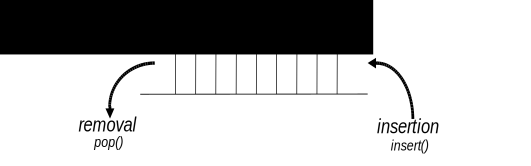
\includegraphics[scale=0.8]{figures/simlib-queue}
    \caption{cQueue: insertion and removal}
    \label{fig:ch-sim-lib:cqueue}
  \end{center}
\end{figure}

The member functions dealing with insertion and removal are
\ffunc{insert()} and \ffunc{pop()}.

\begin{cpp}
cQueue queue("my-queue");
cMessage *msg;

// insert messages
for (int i = 0; i < 10; i++) {
    msg = new cMessage;
    queue.insert(msg);
}

// remove messages
while(!queue.empty()) {
    msg = (cMessage *)queue.pop();
    delete msg;
}
\end{cpp}

The \ffunc{length()} member function returns the number of items in the
queue, and \ffunc{empty()} tells whether there is anything in the queue.

There are other functions dealing with insertion and removal.  The
\ffunc{insertBefore()} and \ffunc{insertAfter()} functions insert a
new item exactly before or after a specified one, regardless of the
ordering function.

The \ffunc{front()} and \ffunc{back()} functions return pointers to the objects
at the front and back of the queue, without affecting queue contents.

The \ffunc{pop()} function can be used to remove items from the
tail of the queue, and the \ffunc{remove()} function can be
used to remove any item known by its pointer from the queue:

\begin{cpp}
queue.remove(msg);
\end{cpp}



\subsubsection{Priority Queue}


By default, \cclass{cQueue} implements a FIFO, but it can also act as
a priority queue, that is, it can keep the inserted objects
ordered\index{queue!order}.  If you want to use this feature, you have
to provide a function that takes two \cclass{cObject} pointers,
compares the two objects and returns -1, 0 or 1 as the result (see the
reference for details).  An example of setting up an ordered
\cclass{cQueue}:

\begin{cpp}
cQueue queue("queue", someCompareFunc);
\end{cpp}


If the queue object is set up as an ordered queue, the \ffunc{insert()}
function uses the ordering function: it searches the queue contents
from the head until it reaches the position where the new item
needs to be inserted, and inserts it there.


\subsubsection{Iterators}


Normally, you can only access the objects at the head or tail of the
queue. However, if you use an iterator class, \cclass{cQueue::Iterator},
you can examine each object in the queue\index{queue!iteration}.

The \cclass{cQueue::Iterator} constructor takes two arguments; the first
is the queue object and the second argument specifies the initial position
of the iterator: 0=tail, 1=head. Otherwise it acts as any other
{\opp} iterator class: you can use the \texttt{++} and \texttt{--} operators to advance
it, the () operator to get a pointer to the current item, and the
\ffunc{end()} member function to examine if you are at the end (or the
beginning) of the queue.


An example:

\begin{cpp}
for( cQueue::Iterator iter(queue,1); !iter.end(), iter++)
{
  cMessage *msg = (cMessage *) iter();
  //...
}
\end{cpp}




\subsection{Expandable Array: cArray}

\subsubsection{Basic Usage}


\cclass{cArray} is a container class that holds objects derived from
\cclass{cObject}. \cclass{cArray} stores the pointers of the objects
inserted instead of making copies. \cclass{cArray} works as an array,
but it grows automatically when it becomes full. Internally,
\cclass{cArray} is implemented with an array of pointers; when the array
fills up, it is reallocated.

\cclass{cArray} objects are used in {\opp} to store parameters
attached to messages, and internally, for storing module parameters
and gates.


Creating an array:

\begin{cpp}
cArray array("array");
\end{cpp}

Adding an object at the first free index:

\begin{cpp}
cPar *p = new cMsgPar("par");
int index = array.add( p );
\end{cpp}


Adding an object at a given index (if the index is occupied,
you will get an error message):

\begin{cpp}
cPar *p = new cMsgPar("par");
int index = array.addAt(5,p);
\end{cpp}


Finding an object in the array:

\begin{cpp}
int index = array.find(p);
\end{cpp}

Getting a pointer to an object at a given index:

\begin{cpp}
cPar *p = (cPar *) array[index];
\end{cpp}

You can also search the array or get a pointer to an object by
the object's name:

\begin{cpp}
int index = array.find("par");
Par *p = (cPar *) array["par"];
\end{cpp}


You can remove an object from the array by calling \ffunc{remove()}
with the object name, the index position or the object pointer:

\begin{cpp}
array.remove("par");
array.remove(index);
array.remove( p );
\end{cpp}


The \ffunc{remove()} function doesn't deallocate the object, but it
returns the object pointer. If you also want to deallocate it, you can
write:

\begin{cpp}
delete array.remove( index );
\end{cpp}

\subsubsection{Iteration}


\cclass{cArray} has no iterator, but it is easy to loop through all the
indices with an integer variable. The \ffunc{size()} member function
returns the largest index plus one.

\begin{cpp}
for (int i = 0; i < array.size(); i++) {
  if (array[i]) { // is this position used?
    cObject *obj = array[i];
    EV << obj->getName() << endl;
  }
}
\end{cpp}


%FIXME document: cXMLElement
%FIXME document: simulation.getUniqueNumber(), for generating unique IDs for models


\section{Routing Support: cTopology}

\subsection{Overview}

The \cclass{cTopology} class was designed primarily to support
routing\index{routing support} in telecommunication or multiprocessor
networks.

A \cclass{cTopology} object stores an abstract representation of the
network in graph form:
\begin{itemize}
  \item{each \cclass{cTopology} node corresponds to a \textit{module}
    (simple or compound), and}
  \item{each \cclass{cTopology} edge corresponds to a \textit{link} or
    \textit{series of connecting links}.}
\end{itemize}

You can specify which modules (either simple or compound) you want to
include in the graph. The graph will include all connections among the
selected modules. In the graph, all nodes are at the same level;
there is no submodule nesting.  Connections which span across compound
module boundaries are also represented as one graph edge. Graph edges
are directed, just as module gates are.


If you are writing a router or switch model, the \cclass{cTopology}
graph can help you determine what nodes are available through which
gate and also to find optimal routes\index{optimal routes}. The
\cclass{cTopology} object can calculate shortest paths\index{shortest
  path} between nodes for you.

The mapping between the graph (nodes, edges) and network model
(modules, gates, connections) is preserved: you can easily find
the corresponding module for a \cclass{cTopology} node and vica versa.





\subsection{Basic Usage}

You can extract the network topology into a \cclass{cTopology}
object by a single function call. You have several ways to select
which modules you want to include in the topology:
\begin{itemize}
  \item{by module type}
  \item{by a parameter's presence and its value}
  \item{with a user-supplied boolean function}
\end{itemize}

First, you can specify which node types you want to include. The
following code extracts all modules of type \ttt{Router} or \ttt{Host}.
(\ttt{Router} and \ttt{Host} can be either simple or compound module types.)

\begin{cpp}
cTopology topo;
topo.extractByModuleType("Router", "Host", nullptr);
\end{cpp}

Any number of module types can be supplied; the list must be terminated by \ttt{nullptr}.

A dynamically assembled list of module types can be passed as a
\ttt{nullptr}-terminated array of \ttt{const char*} pointers, or
in an STL string vector \ttt{std::vector<std::string>}.
An example for the former:

\begin{cpp}
cTopology topo;
const char *typeNames[3];
typeNames[0] = "Router";
typeNames[1] = "Host";
typeNames[2] = nullptr;
topo.extractByModuleType(typeNames);
\end{cpp}

Second, you can extract all modules which have a certain parameter:

\begin{cpp}
topo.extractByParameter( "ipAddress" );
\end{cpp}

You can also specify that the parameter must have a certain value
for the module to be included in the graph:

\begin{cpp}
cMsgPar yes = "yes";
topo.extractByParameter( "includeInTopo", &yes );
\end{cpp}

The third form allows you to pass a function which can determine for
each module whether it should or should not be included.  You can have
\cclass{cTopology} pass supplemental data to the function through a
\ttt{void*} pointer. An example which selects all top-level modules (and
does not use the \ttt{void*} pointer):

\begin{cpp}
int selectFunction(cModule *mod, void *)
{
  return mod->getParentModule() == simulation.getSystemModule();
}

topo.extractFromNetwork( selectFunction, nullptr );
\end{cpp}

%
% TBD one more example which \textit{does use} the void* ptr.
%

A \cclass{cTopology} object uses two types: \cclass{cTopology::Node} for
nodes and \cclass{cTopology::Link} for edges. (\cclass{sTopo\-Link\-In} and
\cclass{cTopology::LinkOut} are `aliases' for \cclass{cTopology::Link}; we'll
talk about them later.)

Once you have the topology extracted, you can start exploring
it. Consider the following code (we'll explain it shortly):

\begin{cpp}
for (int i = 0; i < topo.getNumNodes(); i++) {
  cTopology::Node *node = topo.getNode(i);
  EV << "Node i=" << i << " is " << node->getModule()->getFullPath() << endl;
  EV << " It has " << node->getNumOutLinks() << " conns to other nodes\n";
  EV << " and " << node->getNumInLinks() << " conns from other nodes\n";

  EV << " Connections to other modules are:\n";
  for (int j = 0; j < node->getNumOutLinks(); j++) {
    cTopology::Node *neighbour = node->getLinkOut(j)->getRemoteNode();
    cGate *gate = node->getLinkOut(j)->getLocalGate();
    EV << " " << neighbour->getModule()->getFullPath()
       << " through gate " << gate->getFullName() << endl;
  }
}
\end{cpp}

The \ffunc{getNumNodes()} member function (1st line) returns the number of
nodes in the graph, and getNode(i) returns a pointer to the \textit{i}th
node, an \cclass{cTopology::Node} structure.


The correspondence between a graph node and a module can be obtained
by:

\begin{cpp}
cTopology::Node *node = topo.getNodeFor(module);
cModule *module = node->getModule();
\end{cpp}


The \ffunc{getNodeFor()} member function returns a pointer to the graph
node for a given module. (If the module is not in the graph, it
returns \ttt{nullptr}). \ffunc{getNodeFor()} uses binary search within the
\cclass{cTopology} object so it is relatively fast.


\cclass{cTopology::Node}'s other member functions let you determine the
connections of this node: \ffunc{getNumInLinks()}, \ffunc{getNumOutLinks()} return
the number of connections, \ttt{in(i)} and
\ttt{out(i)} return pointers to graph edge objects.


By calling member functions of the graph edge object, you can
determine the modules and gates involved. The \ffunc{getRemoteNode()}
function returns the other end of the connection, and
\ffunc{getLocalGate()}, \ffunc{getRemoteGate()}, \ffunc{getLocalGateId()} and
\ffunc{getRemoteGateId()} return the gate pointers and ids of the gates
involved. (Actually, the implementation is a bit tricky here: the same
graph edge object \cclass{cTopology::Link} is returned either as
\cclass{cTopology::LinkIn} or as \cclass{cTopology::LinkOut} so that ``remote''
and ``local'' can be correctly interpreted for edges of both
directions.)





\subsection{Shortest Paths}

The real power of \cclass{cTopology} is in finding shortest
paths\index{topology!shortest path} in the network to support optimal
routing\index{optimal routing}. \cclass{cTopology} finds shortest paths
from \textit{all} nodes \textit{to} a target node. The algorithm is
computationally inexpensive. In the simplest case, all edges are
assumed to have the same weight.

A real-life example assumes we have the target module pointer; finding
the shortest path to the target looks like this:

\begin{cpp}
cModule *targetmodulep =...;
cTopology::Node *targetnode = topo.getNodeFor( targetmodulep );
topo.calculateUnweightedSingleShortestPathsTo( targetnode );
\end{cpp}


This performs the Dijkstra algorithm\index{Dijkstra algorithm} and
stores the result in the \cclass{cTopology} object. The result can
then be extracted using \cclass{cTopology} and
\ttt{cTopology::Node}\index{cTopology::Node} methods.  Naturally, each call to
\ffunc{calculateUnweightedSingleShortestPathsTo()} overwrites the results of
the previous call.

Walking along the path from our module to the target node:

\begin{cpp}
cTopology::Node *node = topo.getNodeFor( this );

if (node == nullptr) {
  ev < "We (" << getFullPath() << ") are not included in the topology.\n";
}
else if (node->getNumPaths()==0) {
  EV << "No path to destination.\n";
}
else {
  while (node != topo.getTargetNode()) {
    EV << "We are in " << node->getModule()->getFullPath() << endl;
    EV << node->getDistanceToTarget() << " hops to go\n";
    EV << "There are " << node->getNumPaths()
       << " equally good directions, taking the first one\n";
    cTopology::LinkOut *path = node->getPath(0);
    EV << "Taking gate " << path->getLocalGate()->getFullName()
       << " we arrive in " << path->getRemoteNode()->getModule()->getFullPath()
       << " on its gate " << path->getRemoteGate()->getFullName() << endl;
    node = path->getRemoteNode();
  }
}
\end{cpp}

The purpose of the \ffunc{getDistanceToTarget()} member function of a
node is self-explanatory. In the unweighted case, it returns the
number of hops. The \ffunc{getNumPaths()} member function returns the number
of edges which are part of a shortest path, and
\ffunc[path()]{path(i)} returns the \textit{i}th edge of them as
\cclass{cTopology::LinkOut}. If the shortest paths were created by the
\ffunc[SingleShortestPaths()]{...SingleShortestPaths()} function,
\ffunc{getNumPaths()} will always return 1 (or 0 if the target is not
reachable), that is, only one of the several possible shortest paths
are found.  The
\ffunc[MultiShortestPathsTo()]{...MultiShortestPathsTo()} functions
find all paths, at increased run-time cost. The \cclass{cTopology}'s
\ffunc{getTargetNode()} function returns the target node of the last
shortest path search.

You can enable/disable nodes or edges in the graph. This is done by
calling their \ffunc{enable()} or \ffunc{disable()} member functions.
Disabled nodes or edges are ignored by the shortest paths calculation
algorithm. The \ffunc{isEnabled()} member function returns the state of
a node or edge in the topology graph.

One usage of \ffunc{disable()} is when you want to determine in how many
hops the target node can be reached from our node \textit{through
a particular output gate}. To compute this, you compute the
shortest paths to the target \textit{from the neighbor node} while
disabling the current node to prevent the shortest paths
from going through it:

\begin{cpp}
cTopology::Node *thisnode = topo.getNodeFor(this);
thisnode->disable();
topo.calculateUnweightedSingleShortestPathsTo(targetnode);
thisnode->enable();

for (int j = 0; j < thisnode->getNumOutLinks(); j++) {
  cTopology::LinkOut *link = thisnode->getLinkOut(i);
  EV << "Through gate " << link->getLocalGate()->getFullName() << " : "
     << 1 + link->getRemoteNode()->getDistanceToTarget() << " hops" << endl;
}
\end{cpp}

In the future, other shortest path algorithms will also be implemented:

\begin{cpp}
unweightedMultiShortestPathsTo(cTopology::Node *target);
weightedSingleShortestPathsTo(cTopology::Node *target);
weightedMultiShortestPathsTo(cTopology::Node *target);
\end{cpp}



\section{Pattern Matching}

Since version 4.3, {\opp} contains two utility classes for pattern
matching, \cclass{cPatternMatcher} and \cclass{cMatchExpression}.

\cclass{cPatternMatcher} is a glob-style pattern matching class, adopted to
special {\opp} requirements. It recognizes wildcards, character ranges and
numeric ranges, and supports options such as case sensitive and whole
string matching. \cclass{cMatchExpression} builds on top of
\cclass{cPatternMatcher} and extends it in two ways: first, it lets you
combine patterns with AND, OR, NOT into boolean expressions, and second, it
applies the pattern expressions to \textit{objects} instead of text. These
classes are especially useful for making model-specific configuration files
more concise or more powerful by introducing patterns.

% See \ref{sec:ch-config-sim:wildcards} too.


\subsection{cPatternMatcher}

\cclass{cPatternMatcher} holds a pattern string and several option flags, and has
a boolean \ffunc{matches()} function that lets you check whether the string passed as argument
matches the pattern with the given flags. The pattern and the flags can be set
via the constructor or by calling the \ffunc{setPattern()} member function.

The pattern syntax is a variation on Unix \textit{glob}-style patterns. The
most apparent differences to globbing rules are the distinction between
\ttt{*} and \ttt{**}, and that character ranges should be written with
curly braces instead of square brackets; that is, \textit{any-letter} is
expressed as \ttt{\{a-zA-Z\}} and not as \ttt{[a-zA-Z]}, because square
brackets are reserved for the notation of module vector indices.

The following option flags are supported:

\begin{itemize}
  \item \textit{dottedpath}: controls whether some wildcards (\ttt{?}, \ttt{*}) will match dots
  \item \textit{fullstring}: controls whether to do full string or substring match.
  \item \textit{casesensitive}: whether matching is case sensitive or case insensitive
\end{itemize}

Patterns may contain the following elements:

\begin{itemize}
  \item \textit{question mark}, \ttt{?} : matches any character (except dot if \textit{dottedpath}=true)
  \item \textit{asterisk}, \ttt{*} : matches zero or more characters (except dots if \textit{dottedpath}=true)
  \item \textit{double asterisk}, \ttt{**} : matches zero or more characters, including dots
  \item \textit{set}, e.g. \ttt{\{a-zA-Z\}} : matches any character that is contained in the set
  \item \textit{negated set}, e.g. \ttt{\{{\textasciicircum}a-z\}}: matches any character that is NOT contained in the set
  \item \textit{numeric range}, e.g. \ttt{\{38..150\}} : matches any number (i.e. sequence of digits) in the given range
  \item \textit{numeric index range}, e.g. \ttt{[38..150]} : matches any number in square brackets in the given range
  \item \textit{backslash}, {\textbackslash} : takes away the special meaning of the subsequent character
\end{itemize}

\begin{note}
The \textit{dottedpath} option was introduced to make matching {\opp}
module paths more powerful. When it is off (\textit{dottedpath}=false),
there is no difference between \ttt{*} and \ttt{**}, they both match any
character sequence. However, when matching {\opp} module paths or other
strings where dot is a separator character, it is useful to turn on the
dottedpath mode (\textit{dottedpath}=true). In that mode, \ttt{*}, not
being able to cross a dot, can match only a single path component (or part
of it), and \ttt{**} can match multiple path components.
\end{note}

Sets and negated sets can contain several character ranges and also
enumeration of characters, for example \ttt{\{\_a-zA-Z0-9\}} or
\ttt{\{xyzc-f\}}. To include a hyphen in the set, place it at a position
where it cannot be interpreted as character range, for example
\ttt{\{a-z-\}} or \ttt{\{-a-z\}}. If you want to include a close brace in
the set, it must be the first character: \ttt{\{\}a-z\}}, or for a negated
set: \ttt{\{\textasciicircum\}a-z\}}. A backslash is always taken as
literal backslash (and NOT as escape character) within set definitions.
When doing case-insensitive match, avoid ranges that include both alpha and
non-alpha characters, because they might cause funny results.

For numeric ranges and numeric index ranges, ranges are inclusive, and both
the start and the end of the range are optional; that is, \ttt{\{10..\}},
\ttt{\{..99\}} and \ttt{\{..\}} are all valid numeric ranges (the last one
matches any number). Only nonnegative integers can be matched. Caveat:
\ttt{\{17..19\}} will match \ttt{"a17"}, \ttt{"117"} and also \ttt{"963217"}!

The \cclass{cPatternMatcher} constructor and the \ffunc{setPattern()} member
function have similar signatures:

\begin{cpp}
cPatternMatcher(const char *pattern, bool dottedpath, bool fullstring,
                bool casesensitive);
void setPattern(const char *pattern, bool dottedpath, bool fullstring,
                bool casesensitive);
\end{cpp}

The matcher function:

\begin{cpp}
bool matches(const char *text);
\end{cpp}

There are also some more utility functions for printing the pattern,
determining whether a pattern contains wildcards, etc.

Example:

\begin{cpp}
cPatternMatcher matcher("**.host[*]", true, true, true);
EV << matcher.matches("Net.host[0]") << endl;  // -> true
EV << matcher.matches("Net.area1.host[0]") << endl;  // -> true
EV << matcher.matches("Net.host") << endl;  // -> false
EV << matcher.matches("Net.host[0].tcp") << endl;  // -> false
\end{cpp}


\subsection{cMatchExpression}

The \cclass{cMatchExpression} class builds on top of \cclass{cPatternMatcher},
and lets you determine whether an \textit{object} matches a given pattern
expression.

A pattern expression consists of elements in the
\textit{fieldname(pattern)} syntax; they check whether the string
representation of the given field of the object matches the pattern. For
example, \ttt{srcAddr(192.168.0.*)} will match if the \textit{srcAddr}
field of the object starts with \ttt{192.168.0.} A naked pattern (without
field name and parens) is also accepted, and it will be matched against the
\textit{default field} of the object, which will usually be its name.

These elements can be combined with the AND, OR, NOT operators, accepted in
both lowercase and uppercase. AND has higher precedence than OR, but
parentheses can be used to change the evaluation order.

Pattern examples:

\begin{itemize}
 \item \ttt{"node*"}
 \item \ttt{"node* or host*"}
 \item \ttt{"packet-* and className(PPPFrame)"}
 \item \ttt{"className(TCPSegment) and byteLength(\{4096..\})"}
 \item \ttt{"className(TCPSegment) and (SYN or DATA-*) and not kind(\{0..2\})"}
\end{itemize}

The \cclass{cMatchExpression} class has a constructor and \ffunc{setPattern()}
method similar to those of \cclass{cPatternMatcher}:

\begin{cpp}
cMatchExpression(const char *pattern, bool dottedpath, bool fullstring,
                bool casesensitive);
void setPattern(const char *pattern, bool dottedpath, bool fullstring,
                bool casesensitive);
\end{cpp}

However, the matcher function takes a \cclass{cMatchExpression::Matchable}
instead of string:

\begin{cpp}
bool matches(const Matchable *object);
\end{cpp}

This means that objects to be matched must either be subclassed from
\cclass{cMatchExpression::Matchable}, or be wrapped into some adapter class
that does. \cclass{cMatchExpression::Matchable} is a small abstract class
with only a few pure virtual functions:

\begin{cpp}
/**
 * Objects to be matched must implement this interface
 */
class SIM_API Matchable
{
  public:
    /**
     * Return the default string to match. The returned pointer will not be
     * cached by the caller, so it is OK to return a pointer to a static buffer.
     */
    virtual const char *getAsString() const = 0;

    /**
     * Return the string value of the given attribute, or nullptr if the object
     * doesn't have an attribute with that name. The returned pointer will not
     * be cached by the caller, so it is OK to return a pointer to a static buffer.
     */
    virtual const char *getAsString(const char *attribute) const = 0;

    /**
     * Virtual destructor.
     */
    virtual ~Matchable() {}
};
\end{cpp}

To be able to match instances of an existing class that is not already a
\ttt{Matchable}, you need to write an adapter class. An adapter class that
we can look at as an example is \cclass{cMatchableString}. \cclass{cMatchableString}
makes it possible to match strings with a \cclass{cMatchExpression}, and is part
of {\opp}:

\begin{cpp}
/**
 * Wrapper to make a string matchable with cMatchExpression.
 */
class cMatchableString : public cMatchExpression::Matchable
{
  private:
    std::string str;
  public:
    cMatchableString(const char *s) {str = s;}
    virtual const char *getAsString() const {return str.c_str();}
    virtual const char *getAsString(const char *name) const {return nullptr;}
};
\end{cpp}

An example:

\begin{cpp}
cMatchExpression expr("foo* or bar*", true, true, true);
cMatchableString str1("this is a foo");
cMatchableString str2("something else");
EV << expr.matches(&str1) << endl; // -> true
EV << expr.matches(&str2) << endl; // -> false
\end{cpp}

Or, by using temporaries:

\begin{cpp}
EV << expr.matches(&cMatchableString("this is a foo")) << endl; // -> true
EV << expr.matches(&cMatchableString("something else")) << endl; // -> false
\end{cpp}



\section{Statistics and Distribution Estimation}
\label{sec:ch-sim-lib:statistics}

\subsection{cStatistic and Descendants}

There are several statistic and result collection classes:
\cclass{cStdDev}, \cclass{cWeightedStdDev}, \cclass{Long\-Histogram},
\cclass{cDoubleHistogram}, \cclass{cVarHistogram}, \cclass{cPSquare} and
\cclass{cKSplit}. They are all derived from the abstract base class
\cclass{cStatistic}.

\begin{itemize}
  \item{\cclass{cStdDev} keeps the count, mean, standard
    deviation, minimum and maximum value etc of the observations.}
  \item{\cclass{cWeightedStdDev} is similar to \cclass{cStdDev}, but
    accepts weighted observations. \cclass{cWeightedStdDev} can be used
    for example to calculate time average. It is the only weighted
    statistics class.}
  \item{\cclass{cLongHistogram} and \cclass{cDoubleHistogram} are
    descendants of \cclass{cStdDev} and also keep an approximation of
    the distribution of the observations using equidistant
    (equal-sized) cell histograms\index{histogram!equal-sized}.}
  \item{\cclass{cVarHistogram} implements a histogram where cells do not
    need to be the same size. You can manually add the cell (bin)
    boundaries, or alternatively, automatically have a partitioning
    created where each bin has the same number of observations (or as
    close to that as possible).}
  \item{\cclass{cPSquare} is a class that uses the $P^{2}$ algorithm
    described in \cite{JCh85}. The algorithm calculates quantiles without
    storing the observations; one can also think of it as a histogram
    with equiprobable cells\index{histogram!equiprobable-cells}.}
  \item{\cclass{cKSplit} uses a novel, experimental method, based on an
    adaptive histogram-like algorithm.}
\end{itemize}

\begin{figure}[htbp]
  \begin{center}
    \includegraphics[height=6cm]{figures/cstatistic-inheritance}
    \caption{Statistics classes}
  \end{center}
\end{figure}

\subsubsection{Basic Usage}

One can insert an observation into a statistic object with the
\ffunc{collect()} function or the \texttt{+=} operator (they are
equivalent).  \cclass{cStdDev} has the following methods for getting
statistics from the object: \ffunc{getCount()}, \ffunc{getMin()},
\ffunc{getMax()}, \ffunc{getMean()}, \ffunc{getStddev()}, \ffunc{getVariance()},
\ffunc{getSum()}, \ffunc{getSqrSum()} with the obvious meanings. An example
usage for \cclass{cStdDev}:

\begin{cpp}
cStdDev stat("stat");

for (int i = 0; i < 10; i++)
  stat.collect( normal(0,1) );

long numSamples = stat.getCount();
double smallest = stat.getMin(),
       largest = stat.getMax();
double mean = stat.getMean(),
       standardDeviation = stat.getStddev(),
       variance = stat.getVariance();
\end{cpp}





\subsection{Distribution Estimation}

\subsubsection{Initialization and Usage}

% TBD this has to be rewritten at some point... maybe take over examples from Doxygen doc.

The distribution estimation\index{distribution!estimation} classes
(\cclass{cLongHistogram}, \cclass{cDoubleHistogram}, \cclass{cVarHistogram},
\cclass{cPSquare} and \cclass{cKSplit}) are derived from
\cclass{cDensityEstBase}. Distribution estimation classes (except for
\cclass{cPSquare}) assume that the observations are within a range.
You may specify the range explicitly (based on some a-priori information
about the distribution), or you may let the object precollect a number
of observations and determine the range from them.

The following member functions exist for setting up the range
and to specify how many observations should be used for automatically
determining the range (these methods are part of \cclass{cDensityEstBase}):

\begin{cpp}
setRange(lowerBound, upperBound);
setRangeAuto(numPrecollect, rangeExtFactor);
setRangeAutoLower(upperBound, numPrecollect, rangeExtensionFactor);
setRangeAutoUpper(lowerBound, numPrecollect, rangeExtensionFactor);
\end{cpp}

\begin{cpp}
setNumPrecollectedValues(numPrecollect);
\end{cpp}

The following example creates a histogram with 20 cells and automatic
range estimation\index{histogram!range estimation}:

\begin{cpp}
cDoubleHistogram histogram("histogram", 20);
histogram.setRangeAuto(100,1.5);
\end{cpp}

Here, 20 is the number of cells (not including the underflow/overflow
cells, see later), and 100 is the number of observations to be
collected before setting up the cells. 1.5 is the range extension
factor. It means that the actual range of the initial observations
will be expanded 1.5 times and this expanded range will be used to lay
out the cells. This method increases the chance that further
observations fall in one of the cells and not outside the histogram
range.

\begin{figure}[htbp]
  \begin{center}
    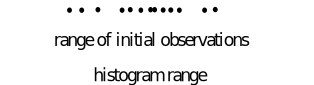
\includegraphics{figures/simlib-histogramrange}
    \caption{Setting up a histogram's range using \ffunc{setRangeAuto()}}
  \end{center}
\end{figure}

The \ffunc{isTransformed()} function returns \textit{true} when the cells have
already been set up. You can force range estimation and setting
up the cells by calling the \ffunc{transform()} function.

The observations that fall outside the histogram range will be counted
as underflows and overflows. The number of underflows and overflows
are returned by the \ffunc{getUnderflowCell()} and \ffunc{getOverflowCell()}
member functions.

\begin{figure}[htbp]
\begin{center}
  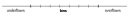
\includegraphics{figures/simlib-histogramsetup}
  \caption{Histogram structure after setting up the cells}
\end{center}
\end{figure}

One exception is the \cclass{cPSquare} class that implements the $P^{2}$
algorithm: it does not use automatic range estimation. The $P^{2}$
algorithm operates by adaptively shifting cell boundaries as observations
arrive, thus, it needs no fixed histogram range. The \ttt{setRange...()}
methods throw an error in \cclass{cPSquare}, and \ffunc{isTransformed()}
always returns \ttt{true}. \cclass{cPSquare} only needs the number of cells
given in, for example in the constructor:

\begin{cpp}
cPSquare psquare("interarrival-times", 20);
\end{cpp}

Afterwards, a \cclass{cPSquare} can be used with the same member functions
as a histogram.


\subsubsection{Querying Histogram Cells}

There are three member functions to explicitly return cell boundaries
and the number of observations in each cell. \ffunc{getNumCells()} returns
the number of cells, \ffunc[getBasepoint()]{getBasepoint(int k)} returns the
\textit{k}th base point, \ffunc[getCellValue()]{getCellValue(int k)} returns the
number of observations in cell \textit{k}, and
\ffunc[getCellPDF()]{getCellPDF(int k)} returns the PDF value in the cell
(i.e. between \ffunc[getBasepoint()]{getBasepoint(k)} and
\ffunc[getBasepoint()]{getBasepoint(k+1)}).
The \ffunc[getCellInfo()]{getCellInfo(k)} method returns multiple data
(cell bounds, counter, relative frequency) packed together in a struct.
These functions work for all histogram types, plus \cclass{cPSquare}
and \cclass{cKSplit}.

\begin{figure}[htbp]
  \begin{center}
    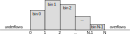
\includegraphics{figures/simlib-histogramcells}
    \caption{Base points and histogram cells}
  \end{center}
\end{figure}

An example:

\begin{cpp}
long n = histogram.getCount();
for (int i = 0; i < histogram.getNumCells(); i++) {
  double cellWidth = histogram.getBasepoint(i+1)-histogram.getBasepoint(i);
  int count = histogram.getCellValue(i);
  double pdf = histogram.getCellPDF(i);
  //...
}
\end{cpp}


The \ffunc[getPDF()]{getPDF(x)} and \ffunc[getCDF()]{getCDF(x)} member functions
return the value of the Probability Density Function and the Cumulated
Density Function at a given \textit{x}, respectively.


\subsubsection{Random Number Generation from Distributions}


The \ffunc{random()} member function generates random
numbers\index{random!numbers} from the distribution stored by the
object:

\begin{cpp}
double rnd = histogram.random();
\end{cpp}


\cclass{cStdDev} assumes normal distribution.

The \cclass{cPar} object stores the pointer to the histogram (or $P^{2}$ object),
and whenever it is asked for the value, calls the histogram object's \ffunc{random()}
function:

\begin{cpp}
double rnd = (double)rndPar; // random number from the cPSquare
\end{cpp}

\subsubsection{Storing and Loading Distributions}


The statistic classes have \ffunc{loadFromFile()} member functions
that read the histogram data from a text file. If you need a custom
distribution\index{distribution!custom} that cannot be written (or it
is inefficient) as a C function, you can describe it in histogram form
stored in a text file, and use a histogram object with
\ffunc{loadFromFile()}.

You can also use \ffunc{saveToFile()}that writes out the distribution
collected by the histogram object:

\begin{cpp}
FILE *f = fopen("histogram.dat","w");
histogram.saveToFile(f); // save the distribution
fclose(f);

cDoubleHistogram hist2("Hist-from-file");
FILE *f2 = fopen("histogram.dat","r");
hist2.loadFromFile(f2); // load stored distribution
fclose(f2);
\end{cpp}


\subsubsection{Histogram with Custom Cells}


The \cclass{cVarHistogram} class can be used to create
histograms with arbitrary (non-equidistant) cells.
It can operate in two modes:

\begin{itemize}
  \item \textit{manual}, where you specify cell boundaries explicitly
     before starting collecting
  \item \textit{automatic}, where \ffunc{transform()} will set up the cells
     after collecting a certain number of initial observations. The cells
     will be set up so that as far as possible, an equal number of observations
     fall into each cell (equi-probable cells).
\end{itemize}

Modes are selected with a \textit{transform-type} parameter:
\begin{itemize}
  \item{\ttt{HIST\_TR\_NO\_TRANSFORM}: no transformation; uses bin boundaries
    previously defined by \ffunc{addBinBound()}}
  \item{\ttt{HIST\_TR\_AUTO\_EPC\_DBL}: automatically creates equiprobable cells}
  \item{\ttt{HIST\_TR\_AUTO\_EPC\_INT}: like the above, but for integers}
\end{itemize}

Creating an object:

\begin{cpp}
cVarHistogram(const char *s=nullptr,
              int numcells=11,
              int transformtype=HIST_TR_AUTO_EPC_DBL);
\end{cpp}

Manually adding a cell boundary:

\begin{cpp}
void addBinBound(double x);
\end{cpp}

Rangemin and rangemax is chosen after collecting the
\texttt{numPrecollect} initial observations. One cannot add cell
boundaries when the histogram has already been transformed.





\subsection{The k-split Algorithm}

\subsubsection{Purpose}


The \textit{k}-split algorithm is an on-line distribution
estimation\index{distribution!online estimation} method.  It was
designed for on-line result collection in simulation programs.  The
method was proposed by Varga and Fakhamzadeh in 1997. The primary
advantage of \textit{k}-split is that without having to store the
observations, it gives a good estimate without requiring a-priori
information about the distribution, including the sample size. The
\textit{k}-split algorithm can be extended to multi-dimensional
distributions\index{distribution!multi-dimensional}, but here we deal
with the one-dimensional version only.


\subsubsection{The Algorithm}


The \textit{k-split} algorithm is an adaptive histogram-type estimate which
maintains a good partitioning by doing cell splits. We start out with
a histogram range $[x_{lo}, x_{hi})$ with $k$ equal-sized histogram
cells with observation counts $n_1,n_2, \cdots n_k$.  Each collected
observation increments the corresponding observation count. When an
observation count $n_i$ reaches a \textit{split threshold}, the cell
is split into $k$ smaller, equal-sized cells with observation counts
$n_{i,1}, n_{i,2}, \cdots n_{i,k}$ initialized to zero. The $n_i$
observation count is remembered and is called the \textit{mother
  observation count} to the newly created cells. Further observations
may cause cells to be split further (e.g. $n_{i,1,1},...n_{i,1,k}$
etc.), thus creating a $k$-order tree of observation counts where
leaves contain live counters that are actually incremented by new
observations, and intermediate nodes contain mother observation counts
for their children. If an observation falls outside the histogram
range, the range is extended in a natural manner by inserting new
level(s) at the top of the tree. The fundamental parameter to the
algorithm is the split factor $k$. Experience has shown that $k=2$
works best.

\begin{figure}[htbp]
  \begin{center}
    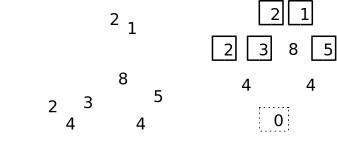
\includegraphics[width=3.442in, height=1.518in]{figures/simlib-ksplit1}
    \caption{Illustration of the k-split algorithm, $k=2$. The
      numbers in boxes represent the observation count values}
  \end{center}
\end{figure}


For density estimation, the total number of observations that
fell into each cell of the partition has to be determined. For
this purpose, mother observations in each internal node of the
tree must be distributed among its child cells and propagated
up to the leaves.

% careful with reformatting! $..$ MUST NOT BE BROKEN TO SEVERAL LINES!

Let $n_{...,i}$ be the (mother) observation count for a cell,
$s_{...,i}$ be the total observation count in a cell $n_{...,i}$ plus
the observation counts in all its sub-, sub-sub-, etc. cells), and
$m_{...,i}$ the mother observations propagated to the cell. We are
interested in the $\tilde{n}_{...,i} = n_{...,i} + m_{...,i}$
estimated amount of observations in the tree nodes, especially in the
leaves. In other words, if we have $\tilde{n}_{...,i}$ estimated
observation amount in a cell, how to divide it to obtain
$m_{...,i,1}, m_{...,i,2} \cdots m_{...,i,k}$
that can be propagated to child cells. Naturally,
$m_{...,i,1} + m_{...,i,2} + \cdots + m_{...,i,k} = \tilde{n}_{...,i}$.

% careful with reformatting! $..$ MUST NOT BE BROKEN TO SEVERAL LINES!

Two natural distribution methods are even
distribution\index{distribution!even} (when
$m_{...,i,1} = m_{...,i,2} = \cdots = m_{...,i,k}$) and proportional
distribution\index{distribution!proportional} (when
$m_{...,i,1} : m_{...,i,2} : \cdots : m_{...,i,k} = s_{...,i,1} : s_{...,i,2} : \cdots : s_{...,i,k}$).
Even distribution is optimal when the
$s_{...,i,j}$ values are very small, and proportional distribution is
good when the $s_{...,i,j}$ values are large compared to
$m_{...,i,j}$. In practice, a linear combination of them seems
appropriate, where $\lambda=0$ means even and $\lambda=1$ means
proportional distribution:

% careful with reformatting! $..$ MUST NOT BE BROKEN TO SEVERAL LINES!

$m_{\cdots,i,j} = (1-\lambda)\tilde{n}_{\cdots,i}/k + \lambda \tilde{n}_{\cdots,i} s_{...,i,j} / s_{\cdots,i}$
where $\lambda\in[0,1]$

\begin{figure}[htbp]
  \begin{center}
    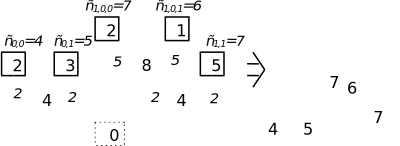
\includegraphics[width=4.147in, height=1.567in]{figures/simlib-ksplit2}
    \caption{Density estimation from the k-split cell tree. We
      assume $\lambda=0$, i.e. we distribute mother observations
      evenly.}
  \end{center}
\end{figure}

% careful with reformatting! $..$ MUST NOT BE BROKEN TO SEVERAL LINES!

Note that while $n_{...,i}$ are integers, $m_{...,i}$ and thus
$\tilde{n}_{...,i}$ are typically real numbers. The histogram estimate
calculated from \textit{k}-split is not exact, because the frequency
counts calculated in the above manner contain a degree of estimation
themselves. This introduces a certain \textit{cell division error};
the $\lambda$ parameter should be selected so that it minimizes that
error. It has been shown that the cell division error can
be reduced to a more-than-acceptable small value.\\
Strictly speaking, the \textit{k}-split algorithm is semi-online,
because its needs some observations to set up the initial histogram
range.  Because of the range extension and cell split
capabilities, the algorithm is not very sensitive to the choice of the
initial range, so very few observations are sufficient for range
estimation (say $N_{pre}=10$). Thus we can regard \textit{k}-split as
an on-line method.

\textit{K}-split can also be used in semi-online mode, when the
algorithm is only used to create an optimal partition from a larger
number of $N_{pre}$ observations. When the partition has been created,
the observation counts are cleared and the $N_{pre}$ observations are
fed into \textit{k}-split once again. This way all mother (non-leaf)
observation counts will be zero and the cell division error is
eliminated. It has been shown that the partition created by
\textit{k}-split can be better than both the equi-distant and the
equal-frequency partition.


{\opp} contains an implementation of the \textit{k}-split algorithm,
the \cclass{cKSplit} class.

\subsubsection{The cKSplit Class}

The \cclass{cKSplit} class is an implementation of the \textit{k-split} method.
Member functions:

%
% TBD comments
%

\begin{cpp}
void setCritFunc(KSplitCritFunc critfunc, double *critdata);
void setDivFunc(KSplitDivFunc divfunc, double *divdata);
void rangeExtension( bool enabled );
\end{cpp}


\begin{cpp}
int getTreeDepth();
int getTreeDepth(cKSplit::Grid& grid);
\end{cpp}

\begin{cpp}
double getRealCellValue(cKSplit::Grid& grid, int cell);
void printGrids();
\end{cpp}

\begin{cpp}
cKSplit::Grid& getGrid(int k);
cKSplit::Grid& getRootGrid();
\end{cpp}

\begin{cpp}
struct cKSplit::Grid
{
  int parent;   // index of parent grid
  int reldepth; // depth = (reldepth - rootgrid's reldepth)
  long total;   // sum of cells & all subgrids (includes "mother")
  int mother;   // observations "inherited" from mother cell
  int cells[K]; // cell values
};
\end{cpp}



\subsection{Transient Detection and Result Accuracy}

In many simulations, only the steady state performance (i.e.
the performance after the system has reached a stable state)
is of interest. The initial part of the simulation is called
the transient period. After the model has entered steady state,
simulation must proceed until enough statistical data has been
collected to compute a result with the required accuracy.


Detection of the end of the transient period and a certain result
accuracy is supported by {\opp}. The user can attach transient
detection\index{transient detection} and result accuracy\index{result
  accuracy} objects to a result object (\cclass{cStatistic}'s
descendants). The transient detection and result accuracy objects will
perform the specific algorithms on the data fed into the result object and
determine if the transient period is over or the result accuracy has been
reached.

The base classes for classes implementing specific transient
detection and result accuracy detection algorithms are:
\begin{itemize}
\item{\cclass{cTransientDetection}: base class for transient detection}
\item{\cclass{cAccuracyDetection}: base class for result accuracy detection}
\end{itemize}


\subsubsection{Basic Usage}

%
% TBD comments
%

Attaching detection objects to a \cclass{cStatistic} and getting pointers
to the attached objects:

\begin{cpp}
addTransientDetection(cTransientDetection *object);
addAccuracyDetection(cAccuracyDetection *object);
cTransientDetection *getTransientDetectionObject();
cAccuracyDetection *getAccuracyDetectionObject();
\end{cpp}


Detecting the end of the period:
\begin{itemize}
\item{polling the \ffunc{detect()} function of the object}
\item{installing a post-detect function}
\end{itemize}


\subsubsection{Transient Detection}


Currently one transient detection\index{transient detection} algorithm
is implemented, i.e.  there is one class derived from
\cclass{cTransientDetection}. The \cclass{cTDExpandingWindows} class
uses the sliding window approach with two windows, and checks the
difference of the two averages to see if the transient period is over.

\begin{cpp}
void setParameters(int reps=3,
                   int minw=4,
                   double wind=1.3,
                   double acc=0.3);
\end{cpp}

\subsubsection{Accuracy Detection}


Currently one accuracy detection\index{accuracy detection} algorithm
is implemented, i.e.  there is one class derived from
\cclass{cAccuracyDetection}. The algorithm implemented in the
\cclass{cADByStddev} class is: divide the standard deviation by the
square of the number of values and check if this is small enough.

\begin{cpp}
void setParameters(double acc=0.1, int reps=3);
\end{cpp}




\section{Recording Simulation Results}
\label{sec:ch-sim-lib:result-recording}

\subsection{Output Vectors: cOutVector}
\label{sec:ch-sim-lib:coutvector}

Objects of type \cclass{cOutVector} are responsible for writing time series
data (referred to as \textit{output vectors}) to a file. The \ffunc{record()}
method is used to output a value (or a value pair) with a timestamp.
The object name will serve as the name of the output vector.

The vector name can be passed in the constructor,

\begin{cpp}
cOutVector responseTimeVec("response time");
\end{cpp}

but in the usual arrangement you'd make the \cclass{cOutVector} a member
of the module class and set the name in \ffunc{initialize()}. You'd
record values from \ffunc{handleMessage()} or from a function called from
\ffunc{handleMessage()}.

The following example is a \ttt{Sink} module which records the lifetime
of every message that arrives to it.

\begin{cpp}
class Sink : public cSimpleModule
{
  protected:
    cOutVector endToEndDelayVec;

    virtual void initialize();
    virtual void handleMessage(cMessage *msg);
};

Define_Module(Sink);

void Sink::initialize()
{
    endToEndDelayVec.setName("End-to-End Delay");
}

void Sink::handleMessage(cMessage *msg)
{
    simtime_t eed = simTime() - msg->getCreationTime();
    endToEndDelayVec.record(eed);
    delete msg;
}
\end{cpp}

There is also a \ffunc{recordWithTimestamp()} method, to make it
possible to record values into output vectors with a timestamp other than
\ffunc{simTime()}. Increasing timestamp order is still enforced though.

All \cclass{cOutVector} objects write to a single \textit{output vector file}
that has a file extension \ttt{.vec}.
  \footnote{A \ttt{.vci} file is also created, but it is just an index for
  the \ttt{.vec} file and does not contain any new information. The IDE
  re-creates the \ttt{.vci} file if it gets lost.}
The format and processing of output vector files is described in section
\ref{cha:analyzing-simulation-results}.

You can configure output vectors from \ffilename{omnetpp.ini}:
you can disable individual vectors, or limit recording to certain
simulation time intervals (section \ref{sec:ana-sim:vector-config}).

If the output vector object is disabled or the simulation time is
outside the specified interval, \ffunc{record()} doesn't write
anything to the output file. However, if you have a Tkenv or Qtenv inspector
window open for the output vector object\index{output!vector object},
the values will be displayed there, regardless of the state of the
output vector object.



\subsection{Output Scalars}

While output vectors are to record time series data and thus they
typically record a large volume of data during a simulation run,
output scalars\index{output!scalars} are supposed to record a single
value per simulation run. You can use output scalars

\begin{itemize}
\item{to record summary data at the end of the simulation run}
\item{to do several runs with different parameter settings/random seed
    and determine the dependence of some measures on the parameter
    settings. For example, multiple runs and output scalars are the
    way to produce \textit{Throughput vs. Offered Load} plots.}
\end{itemize}

Output scalars are recorded with the \ffunc{record()} method of
\cclass{cSimpleModule}, and you will usually want to insert this code
into the \ffunc{finish()} function. An example:

\begin{cpp}
void Transmitter::finish()
{
    double avgThroughput = totalBits / simTime();
    recordScalar("Average throughput", avgThroughput);
}
\end{cpp}

You can record whole statistic objects by calling their \ffunc{record()}
methods, declared as part of \cclass{cStatistic}. In the following example
we create a \ttt{Sink} module which calculates the mean, standard
deviation, minimum and maximum values of a variable, and records them at the
end of the simulation.

\begin{cpp}
class Sink : public cSimpleModule
{
  protected:
    cStdDev eedStats;

    virtual void initialize();
    virtual void handleMessage(cMessage *msg);
    virtual void finish();
};

Define_Module(Sink);

void Sink::initialize()
{
    eedStats.setName("End-to-End Delay");
}

void Sink::handleMessage(cMessage *msg)
{
    simtime_t eed = simTime() - msg->getCreationTime();
    eedStats.collect(eed);
    delete msg;
}

void Sink::finish()
{
    recordScalar("Simulation duration", simTime());
    eedStats.record();
}
\end{cpp}

The above calls record the data into an \textit{output scalar file},
a line-oriented text file that has the file extension \ttt{.sca}.
The format and processing of output vector files is described in chapter
\ref{cha:analyzing-simulation-results}.



\section{Watches and Snapshots}

\subsection{Basic Watches}

Unfortunately, variables of type \ttt{int}, \ttt{long}, \ttt{double}
do not show up by default in Tkenv/Qtenv; neither do STL classes
(\ttt{std::string}, \ttt{std::vector}, etc.) or your own structs and
classes. This is because the simulation kernel, being a library, knows
nothing about types and variables in your source code.

{\opp} provides \fmac{WATCH()} and a set of other macros to
allow variables to be inspectable in Tkenv/Qtenv and to be output into the snapshot
file\index{snapshot file}. \fmac{WATCH()} macros are usually placed into
\ffunc{initialize()} (to watch instance variables) or to the top of the
\ffunc{activity()} function (to watch its local variables); the point being
that they should only be executed once.

\begin{cpp}
long packetsSent;
double idleTime;

WATCH(packetsSent);
WATCH(idleTime);
\end{cpp}

Of course, members of classes and structs can also be watched:

\begin{cpp}
WATCH(config.maxRetries);
\end{cpp}

The Tkenv and Qtenv runtime environments let you inspect and also change
the values of inspected variables.

The \fmac{WATCH()} macro can be used with any type that has a
stream output operator (\ttt{operator<<}) defined. By default,
this includes all primitive types and \ttt{std::string}, but since
you can write \ttt{operator<<} for your classes/structs and basically
any type, \fmac{WATCH()} can be used with anything. The only limitation
is that since the output should more or less fit on single line, the
amount of information that can be conveniently displayed is limited.

An example stream output operator:

\begin{cpp}
std::ostream& operator<<(std::ostream& os, const ClientInfo& cli)
{
    os << "addr=" << cli.clientAddr << "  port=" << cli.clientPort; // no endl!
    return os;
}
\end{cpp}

And the \ttt{WATCH()} line:

\begin{cpp}
WATCH(currentClientInfo);
\end{cpp}


\subsection{Read-write Watches}

Watches for primitive types and \ttt{std::string} allow for changing
the value from the GUI as well, but for other types you need to explicitly
add support for that. What you need to do is define a stream input
operator (\ttt{operator>>}) and use the \fmac{WATCH\_RW()} macro instead of
\fmac{WATCH()}.

The stream input operator:

\begin{cpp}
std::ostream& operator>>(std::istream& is, ClientInfo& cli)
{
    // read a line from "is" and parse its contents into "cli"
    return is;
}
\end{cpp}

And the \ttt{WATCH\_RW()} line:

\begin{cpp}
WATCH_RW(currentClientInfo);
\end{cpp}


\subsection{Structured Watches}

\ttt{WATCH()} and \ttt{WATCH\_RW()} are basic watches; they allow one
line of (unstructured) text to be displayed. However, if you have a
data structure generated from message definitions (see Chapter \ref{cha:messages}),
then there is a better approach. The message compiler automatically generates
meta-information describing individual fields of the class or struct,
which makes it possible to display the contents on field level.

The \texttt{WATCH} macros to be used for this purpose are \fmac{WATCH\_OBJ()}
and \fmac{WATCH\_PTR()}. Both expect the object to be subclassed from
\cclass{cObject}; \fmac{WATCH\_OBJ()} expects a reference to such class,
and \fmac{WATCH\_PTR()} expects a pointer variable.

\begin{cpp}
ExtensionHeader hdr;
ExtensionHeader *hdrPtr;
...
WATCH_OBJ(hdr);
WATCH_PTR(hdrPtr);
\end{cpp}

CAUTION: With \fmac{WATCH\_PTR()}, the pointer variable must point to a valid
object or be \ttt{nullptr} at all times, otherwise the GUI may crash
while trying to display the object. This practically means that
the pointer should be initialized to \ttt{nullptr} even if not used, and
should be set to \ttt{nullptr} when the object to which it points is deleted.

\begin{cpp}
delete watchedPtr;
watchedPtr = nullptr;  // set to nullptr when object gets deleted
\end{cpp}


\subsection{STL Watches}

The standard C++ container classes (\ttt{vector}, \ttt{map}, \ttt{set}, etc)
also have structured watches, available via the following macros:

\fmac{WATCH\_VECTOR()}, \fmac{WATCH\_PTRVECTOR()},
\fmac{WATCH\_LIST()}, \fmac{WATCH\_PTRLIST()},
\fmac{WATCH\_SET()}, \fmac{WATCH\_PTRSET()},
\fmac{WATCH\_MAP()}, \fmac{WATCH\_PTRMAP()}.

The \ttt{PTR}-less versions expect the data items ("T") to have
stream output operators (\ttt{operator <<}), because that is how
they will display them. The \ttt{PTR} versions assume that
data items are pointers to some type which has \ttt{operator <<}.
\fmac{WATCH\_PTRMAP()} assumes that only the value type (``second'')
is a pointer, the key type (``first'') is not. (If you happen to use
pointers as key, then define \ttt{operator <<} for the pointer type
itself.)

Examples:

\begin{cpp}
std::vector<int> intvec;
WATCH_VECTOR(intvec);

std::map<std::string,Command*> commandMap;
WATCH_PTRMAP(commandMap);
\end{cpp}



\subsection{Snapshots}
\label{sec:ch-sim-lib:snapshots}

The \ffunc{snapshot()} function outputs textual information about all
or selected objects of the simulation (including the objects created
in module functions by the user) into the snapshot file\index{snapshot file}.

\begin{cpp}
bool snapshot(cObject *obj = &simulation, const char *label = nullptr);
\end{cpp}

The function can be called from module functions, like this:

\begin{cpp}
snapshot();     // dump the whole network
snapshot(this); // dump this simple module and all its objects
snapshot(&simulation.msgQueue); // dump future events
\end{cpp}

This will append snapshot information to the end of the snapshot file.
(The snapshot file name has an extension of \ttt{.sna}, default is
\ttt{omnetpp.sna}\index{omnetpp.sna}. The actual file name can be set in the
config file.)

The snapshot file output is detailed enough to be used for debugging
the simulation: by regularly calling \ffunc{snapshot()}, one can trace
how the values of variables, objects changed over the simulation.
The arguments: label is a string that will appear in the output
file; obj is the object whose inside is of interest. By default,
the whole simulation (all modules etc) will be written out.

If you run the simulation with Tkenv or Qtenv, you can also create a
snapshot from the menu.

An example snapshot file (some abbreviations have been applied):

\begin{filelisting}
<?xml version="1.0" encoding="ISO-8859-1"?>
<snapshot object="simulation" label="Long queue" simtime="9.038229311343"
network="FifoNet">
  <object class="cSimulation" fullpath="simulation">
    <info></info>
    <object class="cModule" fullpath="FifoNet">
      <info>id=1</info>
      <object class="fifo::Source" fullpath="FifoNet.gen">
        <info>id=2</info>
        <object class="cPar" fullpath="FifoNet.gen.sendIaTime">
          <info>exponential(0.01s)</info>
          <detailedinfo>double sendIaTime = exponential(0.01s) @unit(s)
          </detailedinfo>
        </object>
        <object class="cGate" fullpath="FifoNet.gen.out">
          <info>--&gt; fifo.in</info>
        </object>
      </object>
      <object class="fifo::Fifo" fullpath="FifoNet.fifo">
        <info>id=3</info>
        <object class="cPar" fullpath="FifoNet.fifo.serviceTime">
          <info>0.01</info>
          <detailedinfo>double serviceTime = 0.01@unit(s)</detailedinfo>
        </object>
        <object class="cGate" fullpath="FifoNet.fifo.in">
          <info>&lt;-- gen.out</info>
        </object>
        <object class="cGate" fullpath="FifoNet.fifo.out">
          <info>--&gt; sink.in</info>
        </object>
        <object class="cQueue" fullpath="FifoNet.fifo.queue">
          <info>length=13</info>
          <object class="cMessage" fullpath="FifoNet.fifo.queue.job">
            <info>src=FifoNet.gen (id=2)  dest=FifoNet.fifo (id=3)</info>
          </object>
          <object class="cMessage" fullpath="FifoNet.fifo.queue.job">
            <info>src=FifoNet.gen (id=2)  dest=FifoNet.fifo (id=3)</info>
          </object>
        </object>
      <object class="fifo::Sink" fullpath="FifoNet.sink">
        <info>id=4</info>
        <object class="cGate" fullpath="FifoNet.sink.in">
          <info>&lt;-- fifo.out</info>
        </object>
      </object>
    </object>
    <object class="cMessageHeap" fullpath="simulation.scheduled-events">
      <info>length=3</info>
      <object class="cMessage" fullpath="simulation.scheduled-events.job">
        <info>src=FifoNet.fifo (id=3)  dest=FifoNet.sink (id=4)</info>
      </object>
      <object class="cMessage" fullpath="...sendMessageEvent">
        <info>at T=9.0464.., in dt=0.00817..; selfmsg for FifoNet.gen (id=2)</info>
      </object>
      <object class="cMessage" fullpath="...end-service">
        <info>at T=9.0482.., in dt=0.01; selfmsg for FifoNet.fifo (id=3)</info>
      </object>
    </object>
  </object>
</snapshot>

\end{filelisting}



% \subsection{Disabling Warnings}
%
% Some container classes and functions suspend the simulation and issue
% warning messages in potentially bogus/dangerous situations, for
% example when an object is not found and \ttt{nullptr} pointer/reference is
% about to be returned. Very often this is useful, but sometimes it is
% more trouble. You can turn warnings on/off from the ini file
% (warnings=yes/no)\index{ini file!warnings}.
%
%
% It is a good practice to leave warnings\index{warnings} enabled, and
% temporarily disable warnings in places where {\opp} would normally
% issue warnings but you know the code is correct. This is done in the
% following way:
%
% \ begin{verbatim}
% bool w = simulation.warnings();
% simulation.setWarnings( false );
% ...
% ... // critical code
% ...
% simulation.setWarnings( w );
% \ end{verbatim}





\subsection{Getting Coroutine Stack Usage}

It is important to choose the correct stack size for
modules\index{module!stack size}\index{stack!size}.  If the stack is
too large, it unnecessarily consumes memory; if it is too small, stack
violation occurs.

%From the Feb99 release,
{\opp} contains a mechanism that detects stack
overflows\index{stack!overflow}. It checks the intactness of a
predefined byte pattern (\texttt{0xdeadbeef}) at the stack boundary,
and reports ``stack violation''\index{stack!violation} if it was
overwritten. The mechanism usually works fine, but occasionally it can
be fooled by large -- and not fully used -- local variables (e.g. char
buffer[256]): if the byte pattern happens to fall in the middle of
such a local variable, it may be preserved intact and {\opp} does not
detect the stack violation.

To be able to make a good guess about stack size, you can use
the \ffunc{getStackUsage()} call which tells you how much stack the module
actually uses. It is most conveniently called from \ffunc{finish()}:

\begin{cpp}
void FooModule::finish()
{
  EV << getStackUsage() << " bytes of stack used\n";
}
\end{cpp}


The value includes the extra stack added by the user interface library
(see \textit{extraStackforEnvir}\index{extraStackforEnvir} in
envir/omnetapp.h), which is currently 8K for Cmdenv and at least 16K
for Tkenv.
  \footnote{The actual value is platform-dependent.}

\ffunc{getStackUsage()} also works by checking the existence of predefined
byte patterns in the stack area, so it is also subject to the above
effect with local variables.


\section{Defining New NED Functions}
\label{sec:ch-sim-lib:defining-ned-functions}

It is possible to extend the NED language with new functions beyond the
built-in ones. New functions are implemented in C++, and then compiled into
the simulation model. When a simulation program starts up, the new
functions are registered in the NED runtime, and become available for use
in NED and ini files.

There are two methods to define NED functions. The
\fmac{Define\_NED\_Function()} macro is the more flexible, preferred method
of the two. \fmac{Define\_NED\_Math\_Function()} is the older one, and it
supports only certain cases. Both macros have several variants.
  \footnote{Before {\opp} 4.2, \fmac{Define\_NED\_Math\_Function()} was
  called \fmac{Define\_Function()}.}

\subsection{Define\_NED\_Function()}

The \fmac{Define\_NED\_Function()} macro lets you define new functions that
can accept arguments of various data types (\ttt{bool}, \ttt{double},
\ttt{string}, etc.), supports optional arguments and also variable
argument lists (variadic functions).

The macro has two variants:

\begin{cpp}
Define_NED_Function(FUNCTION,SIGNATURE);
Define_NED_Function2(FUNCTION,SIGNATURE,CATEGORY,DESCRIPTION);
\end{cpp}

The two variants are basically equivalent; the only difference is that the
second one allows you to specify two more parameters, \ttt{CATEGORY} and
\ttt{DESCRIPTION}. These two parameters expect human-readable strings that
are displayed when listing the available NED functions.

The common parameters, \ttt{FUNCTION} and \ttt{SIGNATURE} are the important
ones. \ttt{FUNCTION} is the name of (or pointer to) the C++ function that
implements the NED function, and \ttt{SIGNATURE} is the function signature
as a string; it defines the name, argument types and return type of the NED
function.

You can list the available NED functions by running \fprog{opp\_run} or
any simulation executable with the \ttt{-h nedfunctions} option.
The result will be similar to what you can see in Appendix
\ref{cha:ned-functions}.

\begin{commandline}
$ opp_run -h nedfunctions
OMNeT++ Discrete Event Simulation...
Functions that can be used in NED expressions and in omnetpp.ini:

 Category "conversion":
  double : double double(any x)
    Converts x to double, and returns the result. A boolean argument becomes
    0 or 1; a string is interpreted as number; an XML argument causes an error.
 ...
\end{commandline}

Seeing the above output, it should now be obvious what the \ttt{CATEGORY}
and \ttt{DESCRIPTION} macro arguments are for. {\opp} uses the following
category names: \ttt{"conversion"}, \ttt{"math"}, \ttt{"misc"},
\ttt{"ned"}, \ttt{"random/continuous"}, \ttt{"random/discrete"},
\ttt{"strings"}, \ttt{"units"}, \ttt{"xml"}. You can use these category names
for your own functions as well, when appropriate.


\subsubsection{The Signature}

The signature string has the following syntax:

\begin{Verbatim}[commandchars=\\\{\}]
\textit{returntype functionname(argtype1 argname1, argtype2 argname2, ...)}
\end{Verbatim}

The \textit{functionname} part defines the name of the NED function, and it
must meet the syntactical requirements for NED identifiers (start with a
letter or underscore, not be a reserved NED keyword, etc.)

The argument types and return type can be one of the following:
\fkeyword{bool}, \fkeyword{int} (maps to C/C++ \ttt{long}),
\fkeyword{double}, \fkeyword{quantity}, \fkeyword{string}, \fkeyword{xml}
or \fkeyword{any}; that is, any NED parameter type plus \fkeyword{quantity}
and \fkeyword{any}. \fkeyword{quantity} means \textit{double with an
optional measurement unit} (\fkeyword{double} and \fkeyword{int} only
accept dimensionless numbers), and \fkeyword{any} stands for any type. The
argument names are presently ignored.

To make arguments optional, append a question mark to the argument name.
Like in C++, optional arguments may only occur at the end of the argument
list, i.e. all arguments after an optional argument must also be optional.
The signature string does not have syntax for supplying default values for
optional arguments; that is, default values have to be built into the C++
code that implements the NED function. To let the NED function accept any
number of additional arguments of arbitrary types, add an ellipsis
(\ttt{...}) to the signature as the last argument.

Some examples:

\begin{cpp}
"int factorial(int n)"
"bool isprime(int n)"
"double sin(double x)"
"string repeat(string what, int times)"
"quantity uniform(quantity a, quantity b, long rng?)"
"any choose(int index, ...)"
\end{cpp}

The first three examples define NED functions with the names \ttt{factorial},
\ttt{isprime} and \ttt{sin}, with the obvious meanings. The fourth example
can be the signature for a function that repeats a string $n$ times, and
returns the concatenated result. The fifth example is the signature of the
existing \ttt{uniform()} NED function; it accepts numbers both with and without
measurement units (of course, when invoked with measurement units, both \ttt{a}
and \ttt{b} must have one, and the two must be compatible -- this should be checked
by the C++ implementation). \ttt{uniform()} also accepts an optional third argument,
an RNG index. The sixth example can be the signature of a \ttt{choose()}
NED function that accepts an integer plus any number of additional arguments
of any type, and returns the \textit{index}th one among them.

\subsubsection{Implementing the NED Function}

The C++ function that implements the NED function must have the following
signature, as defined by the \fdef{NEDFunction} typedef:

\begin{cpp}
cNEDValue function(cComponent *context, cNEDValue argv[], int argc);
\end{cpp}

As you can see, the function accepts an array of \cclass{cNEDValue}
objects, and returns a \cclass{cNEDValue}; the \textit{argc-argv} style
argument list should be familiar to you from the declaration of the C/C++
\ttt{main()} function. \cclass{cNEDValue} is a class that is used during
the evaluation of NED expressions, and represents a value together with its
type.  The \ttt{context} argument contains the module or channel in the
context of which the NED expression is being evaluated; it is useful for
implementing NED functions like \ttt{getParentModuleIndex()}.

The function implementation does not need to worry too much about checking
the number and types of the incoming arguments, because the NED expression
evaluator already does that: inside the function you can be sure that the
number and types of arguments correspond to the function signature string.
Thus, \ttt{argc} is mostly useful only if you have optional arguments or a
variable argument list. The NED expression evaluator also checks that the
value you return from the function corresponds to the signature.

\cclass{cNEDValue} can store all the needed data types (\ttt{bool},
\ttt{double}, \ttt{string}, etc.), and is equipped with the functions
necessary to conveniently read and manipulate the stored value. The value can
be read via functions like \ffunc{boolValue()}, \ffunc{longValue()},
\ffunc{doubleValue()}, \ffunc{stringValue()} (returns \ttt{const char *}),
\ffunc{stdstringValue()} (returns \ttt{const std::string\&}) and
\ffunc{xmlValue()} (returns \ttt{cXMLElement*}), or by simply casting the
object to the desired data type, making use of the provided typecast
operators. Invoking a getter or typecast operator that does not match the
stored data type will result in a runtime error. For setting the stored
value, \cclass{cNEDValue} provides a number of overloaded \ffunc{set()}
functions, assignment operators and constructors.

Further \cclass{cNEDValue} member functions provide access to the stored
data type; yet other functions are associated with handling quantities,
i.e. doubles with measurement units. There are member functions for getting
and setting the number part and the measurement unit part separately; for
setting the two components together; and for performing unit conversion.

Equipped with the above information, we can already write a simple NED function
that returns the length of a string:

\begin{cpp}
static cNEDValue ned_strlen(cComponent *context, cNEDValue argv[], int argc)
{
    return (long)argv[0].stdstringValue().size();
}

Define_NED_Function(ned_strlen, "int length(string s)");
\end{cpp}

Note that since \fmac{Define\_NED\_Function()} expects the C++ function to
be already declared, we place the function implementation in front of the
\fmac{Define\_NED\_Function()} line. We also declare the function to be
\ttt{static}, because its name doesn't need to be visible for the linker.
In the function body, we use \ttt{std::string}'s \ttt{size()} method to
obtain the length of the string, and cast the result to \ttt{long}; the C++
compiler will convert that into a \ttt{cNEDValue} using \ttt{cNEDValue}'s
\ttt{long} constructor. Note that the \fkeyword{int} keyword in the signature
maps to the C++ type \ttt{long}.

The following example defines a \ttt{choose()} NED function that returns
its $k$th argument that follows the \ttt{index} ($k$) argument.

\begin{cpp}
static cNEDValue ned_choose(cComponent *context, cNEDValue argv[], int argc)
{
    int index = (int)argv[0];
    if (index < 0 || index >= argc-1)
        throw cRuntimeError("choose(): index %d is out of range", index);
    return argv[index+1];
}

Define_NED_Function(ned_choose, "any choose(int index, ...)");
\end{cpp}

Here, the value of \ttt{argv[0]} is read using the typecast operator that
maps to \ttt{longValue()}. (Note that if the value of the \ttt{index}
argument does not fit into an \ttt{int}, the conversion will result
in data loss!) The code also shows how to report errors (by throwing a
\cclass{cRuntimeError}.)

The third example shows how the built-in \ttt{uniform()} NED function could
be reimplemented by the user:

\begin{cpp}
static cNEDValue ned_uniform(cComponent *context, cNEDValue argv[], int argc)
{
    int rng = argc==3 ? (int)argv[2] : 0;
    double argv1converted = argv[1].doubleValueInUnit(argv[0].getUnit());
    double result = uniform((double)argv[0], argv1converted, rng);
    return cNEDValue(result, argv[0].getUnit());
    // or: argv[0].setPreservingUnit(result); return argv[0];
}

Define_NED_Function(ned_uniform, "quantity uniform(quantity a, quantity b, int rng?)");
\end{cpp}

The first line of the function body shows how to supply default values for
optional arguments; for the \ttt{rng} argument in this case. The next line
deals with unit conversion. This is necessary because the \ttt{a} and
\ttt{b} arguments are both quantities and may come in with different
measurement units. We use the \ffunc{doubleValueInUnit()} function to
obtain the numeric value of \ttt{b} in \ttt{a}'s measurement unit. If the
two units are incompatible or only one of the parameters have a unit, an
error will be raised. If neither parameters have a unit,
\ffunc{doubleValueInUnit()} simply returns the stored \ttt{double}. Then we
call the \ttt{uniform()} C++ function to actually generate a random number,
and return it in a temporary object with \ttt{a}'s measurement unit.
Alternatively, we could have overwritten the numeric part of \ttt{a} with
the result using \ffunc{setPreservingUnit()}, and returned just that. If
there is no measurement unit, \ffunc{getUnit()} will return \ttt{nullptr},
which is understood by both \ffunc{doubleValueInUnit()} and the
\cclass{cNEDValue} constructor.

\begin{note}
Note that it is OK to change the elements of the \ttt{argv[]} vector: they
will be discarded (popped off the evaluation stack) by the NED expression
evaluator anyway when your function returns.
\end{note}


\subsubsection{cNEDValue In More Detail}

In the previous section we have given an overview and demonstrated the basic
use of the \cclass{cNEDValue} class; here we go into further details.

The stored data type can be obtained with the \ffunc{getType()} function.
It returns an enum (\ttt{cNEDValue::Type}) that has the following values:
\ttt{UNDEF}, \ttt{BOOL}, \ttt{DBL}, \ttt{STR}, \ttt{XML}. \ttt{UNDEF} is
synonymous with \textit{unset}; the others have the obvious meanings. There
is no separate \ttt{QUANTITY} type: quantities are also represented with
the \ttt{DBL} type, which has an optional associated measurement unit. Note
that \ttt{LONG} is also missing; the reason is that the NED expression
evaluator currently (as of {\opp} 4.2) stores all numbers as \ttt{double}s.
  \footnote{The IEEE \textit{double}'s mantissa is 53 bits, so \ttt{double}
  can accurately represent 32-bit integers, the usual size of \ttt{long} on
  32-bit architectures. On 64-bit architectures the usual size of \ttt{long}
  is 64 bits, so precision loss will occur when converting very large integers
  to \ttt{double}. Note, however, that simulations that trigger this precision
  loss would not be able to run on 32-bit architectures at all!}

The \ffunc{getTypeName()} static function returns the string equivalent of
a \ttt{cNEDValue::Type}. The utility functions \ffunc{isSet()} and
\ffunc{isNumeric()} check that the type is (not) \ttt{UNDEF} and \ttt{DBL},
respectively.

\begin{cpp}
cNEDValue value = 5.0;
cNEDValue::Type type = value.getType(); // ==> DBL
EV << cNEDValue::getTypeName(type) << endl; // ==> "double"
\end{cpp}

We have already seen that the \ttt{DBL} type serves both the
\fkeyword{double} and \fkeyword{quantity} types of the NED function
signature, by storing an optional measurement unit (a string)
in addition to the \ttt{double} variable. A \cclass{cNEDValue} can be set
to a quantity by creating it with a two-argument constructor that accepts
a \ttt{double} and a \ttt{const char *} for unit, or by invoking a similar
two-argument \ffunc{set()} function. The measurement unit can be read with
\ffunc{getUnit()}, and overwritten with \ffunc{setUnit()}. If you assign a
\ttt{double} to a \cclass{cNEDValue} or invoke the one-argument
\ttt{set(double)} method on it, that will clear the measurement unit. If you
want to overwrite the number part but preserve the original unit, you need
to use the \ffunc{setPreservingUnit(double)} method.

There are several functions that perform unit conversion. The
\ffunc{doubleValueInUnit()} method accepts a measurement unit, and attempts
to return the number in that unit. The \ffunc{convertTo()} method also
accepts a measurement unit, and tries to permanently convert the value to
that unit; that is, if successful, it changes both the number and the
measurement unit part of the object. The \ffunc{convertUnit()} static
\cclass{cNEDValue} member function accepts three arguments: a quantity as a
\ttt{double} and a unit, and a target unit; and returns the number in the
target unit. A \ffunc{parseQuantity()} static member function parses
a string that contains a quantity (e.g. \ttt{"5min 48s"}), and return
both the numeric value and the measurement unit. Another version of
\ffunc{parseQuantity()} tries to return the value in a unit you specify.
All functions raise an error if the unit conversion is not possible, e.g.
due to incompatible units.

For performance reasons, \ttt{setUnit()}, \ttt{convertTo()} and all other
functions that accept and store a measurement unit will only store the
\ttt{const char*} pointer, but do \textit{not} copy the string itself.
Consequently, the passed measurement unit pointers must stay valid for at
least the lifetime of the \cclass{cNEDValue} object, or even longer if the
same pointer propagates to other \cclass{cNEDValue} objects. It is
recommended that you only pass pointers that stay valid during the entire
simulation. It is safe to use: (1) string constants from the code; (2) unit
strings from other \cclass{cNEDValue}s; and (3) pooled strings e.g. from a
\cclass{cStringPool} or from \cclass{cNEDValue}'s static \ffunc{getPooled()}
function.

Example code:

\begin{cpp}
// manipulating the number and the measurement unit
cNEDValue value(250,"ms");    // initialize to 250ms
value = 300.0;                // ==> 300 (clears the unit!)
value.set(500,"ms");          // ==> 500ms
value.setUnit("s");           // ==> 500s (overwrites the unit)
value.setPreservingUnit(180); // ==> 180s (overwrites the number)
value.setUnit(nullptr);       // ==> 180 (clears the unit)

// unit conversion
value.set(500, "ms");         // ==> 500ms
value.convertTo("s");         // ==> 0.5s
double us = value.doubleValueInUnit("us"); // ==> 500000 (value is unchanged)
double bps = cNEDValue::convertUnit(128, "kbps", "bps"); // ==> 128000
double ms = cNEDValue::convertUnit("2min 15.1s", "ms"); // ==> 135100

// getting persistent measurement unit strings
const char *unit = argv[0].stringValue(); // cannot be trusted to persist
value.setUnit(cNEDValue::getPooled(unit)); // use a persistent copy for setUnit()
\end{cpp}


\subsection{Define\_NED\_Math\_Function()}

The \fmac{Define\_NED\_Math\_Function()} macro lets you register a C/C++
``mathematical'' function as a NED function. The registered C/C++ function
may take up to four \ttt{double} arguments, and must return a \ttt{double};
the NED signature will be the same. In other words, functions registered
this way cannot accept any NED data type other than \ttt{double}; cannot
return anything else than \ttt{double}; cannot accept or return values with
measurement units; cannot have optional arguments or variable argument
lists; and are restricted to four arguments at most. In exchange for these
restrictions, the C++ implementation of the functions is a lot simpler.

Accepted function signatures for \fmac{Define\_NED\_Math\_Function()}:

\begin{cpp}
double f();
double f(double);
double f(double, double);
double f(double, double, double);
double f(double, double, double, double);
\end{cpp}

The simulation kernel uses \fmac{Define\_NED\_Math\_Function()} to expose
commonly used \ttt{<math.h>} functions in the NED language. Most \ttt{<math.h>}
functions (\ttt{sin()}, \ttt{cos()}, \ttt{fabs()}, \ttt{fmod()}, etc.)
can be directly registered without any need for wrapper code, because their
signatures is already one of the accepted ones listed above.

The macro has the following variants:

\begin{cpp}
Define_NED_Math_Function(NAME,ARGCOUNT);
Define_NED_Math_Function2(NAME,FUNCTION,ARGCOUNT);
Define_NED_Math_Function3(NAME,ARGCOUNT,CATEGORY,DESCRIPTION);
Define_NED_Math_Function4(NAME,FUNCTION,ARGCOUNT,CATEGORY,DESCRIPTION);
\end{cpp}

All macros accept the \ttt{NAME} and \ttt{ARGCOUNT} parameters; they are
the intended name of the NED function and the number of \ttt{double}
arguments the function takes (0..3). \ttt{NAME} should be provided without
quotation marks (they will be added inside the macro.) Two macros also
accept a \ttt{FUNCTION} parameter, which is the name of (or pointer to) the
implementation C/C++ function. The macros that don't have a \ttt{FUNCTION}
parameter simply use the \ttt{NAME} parameter for that as well. The last
two macros accept \ttt{CATEGORY} and \ttt{DESCRIPTION}, which have exactly
the same role as with \fmac{Define\_NED\_Function()}.

Examples:

\begin{cpp}
Define_NED_Math_Function3(sin, 1, "math", "Trigonometric function; see <math.h>");
Define_NED_Math_Function3(cos, 1, "math", "Trigonometric function; see <math.h>");
Define_NED_Math_Function3(pow, 2, "math", "Power-of function; see <math.h>");
\end{cpp}



\section{Deriving New Classes}
\label{sec:ch-sim-lib:deriving-new-classes}

\subsection{cObject or Not?}

If you plan to implement a completely new class (as opposed to
subclassing something already present in {\opp}), you have
to ask yourself whether you want the new class to be based
on \cclass{cObject} or not.
Note that we are \textit{not} saying you should always
subclass from \cclass{cObject}.
Both solutions have advantages and disadvantages, which you
have to consider individually for each class.

\cclass{cObject} already carries (or provides a framework for)
significant functionality that is either relevant to
your particular purpose or not. Subclassing \cclass{cObject}
generally means you have more code to write (as you \textit{have to}
redefine certain virtual functions and adhere to conventions)
and your class will be a bit more heavy-weight.
However, if you need to store your objects in {\opp} objects like \cclass{cQueue}
or you want to store {\opp} classes in your object,
then you \textit{must} subclass from \cclass{cObject}.
  \footnote{For simplicity, in these sections ``{\opp} object''
  should be understood as ``object of a class subclassed from
  \cclass{cObject}''}

The most significant features of \cclass{cObject} are
the name string (which has to be stored somewhere, so it has
its overhead) and ownership management (see section
\ref{sec:ch-sim-lib:ownership-management}), which
also provides advantages at some cost.

As a general rule, small \ttt{struct}-like classes like \ttt{IPAddress} or
\ttt{MACAddress} are better \textit{not} subclassed from \cclass{cObject}.
If your class has at least one virtual member function, consider
subclassing from \cclass{cObject}, which does not impose any
extra cost because it doesn't have data members at all, only
virtual functions.


\subsection{cObject Virtual Methods}

Most classes in the simulation class library are descendants of
\cclass{cObject}. If you want to derive a new class from
\cclass{cObject} or a \cclass{cObject} descendant, you must redefine
some member functions so that objects of the new type can fully
co-operate with other parts of the simulation system. A more or less
complete list of these functions is presented here. You don't need to
worry about the length of the list: most functions are not
absolutely necessary to implement. For example, you do not need to
redefine \ffunc{forEachChild()} unless your class is a container class.

The following methods \textbf{must} be implemented:

\begin{itemize}
  \item{\textit{Constructor}. At least two constructors should be provided:
        one that takes the object name string as \ttt{const char *}
        (recommended by convention), and another one with no arguments
        (must be present). The two are usually implemented as a single
        method, with \ttt{nullptr} as default name string.}
  \item{\textit{Copy constructor}, which must have the following signature
        for a class \ttt{X}: \ttt{X(const X\&)}.}
  \item{\textit{Destructor}.}
  \item{\textit{Duplication function,} \ffunc{X *dup() const}.
        It should create and return an exact duplicate of the object.
        It is usually a one-line function that delegates to the copy constructor.}
  \item{\textit{Assignment operator}, that is, \ttt{X\& operator=(const X\&)}
        for a class \ttt{X}. It should copy the contents of the other
        object into this one, \textit{except} the name string. See later what to do
        if the object contains pointers to other objects.}
\end{itemize}

If your class contains other objects subclassed from \cclass{cObject},
either via pointers or as a data member, the following function \textbf{should}
be implemented:

\begin{itemize}
  \item{\textit{Iteration function,} \ttt{void forEachChild(cVisitor *v)}.
        The implementation should call the function passed
        for each object it contains via pointer or as a data member;
        see the API Reference on \cclass{cObject} on how to implement
        \ttt{forEachChild()}. \ffunc{forEachChild()} makes it possible
        for Tkenv and Qtenv to display the object tree to you, to perform searches on it, etc.
        It is also used by \ffunc{snapshot()} and some other library functions.}
\end{itemize}

Implementation of the following methods is \textbf{recommended}:

\begin{itemize}
  \item{\textit{Object info,} \ffunc{std::string info()}. The \ttt{info()} function
        should return a one-line string describing the object's contents or state.
        \ttt{info()} is displayed at several places in Tkenv and Qtenv.}
  \item{\textit{Detailed object info,} \ffunc{std::string detailedInfo()}.
        This method may potentially be implemented in addition to \ttt{info()};
        it can return a multi-line description. \ttt{detailedInfo()} is also
        displayed by Tkenv ad Qtenv in the object's inspector.}
  \item{\textit{Serialization}, \ffunc{parsimPack()} and \ffunc{parsimUnpack()} methods.
        These methods are needed for parallel simulation, if you want
        objects of this type to be transmitted across partitions.}
\end{itemize}

It is customary to implement the copy constructor and the assignment operator
so that they delegate to the same function of the base class, and invoke a common
private \ffunc{copy()} function to copy the local members.

\subsection{Class Registration}

You should also use the \fmac{Register\_Class()} macro to register the
new class. It is used by the \ffunc{createOne()} factory function, which can
create any object given the class name as a string. \ffunc{createOne()}
is used by the Envir library to implement \ffilename{omnetpp.ini} options
such as \ttt{rng-class="..."} or \ttt{scheduler-class="..."}.
(see Chapter \ref{cha:plugin-exts})

For example, an \ffilename{omnetpp.ini} entry such as

\begin{inifile}
rng-class = "cMersenneTwister"
\end{inifile}

would result in something like the following code to be executed
for creating the RNG objects:

\begin{cpp}
cRNG *rng = check_and_cast<cRNG*>(createOne("cMersenneTwister"));
\end{cpp}

But for that to work, we needed to have the following line somewhere in the code:

\begin{cpp}
Register_Class(cMersenneTwister);
\end{cpp}

\ffunc{createOne()} is also needed by the parallel distributed simulation feature
(Chapter \ref{cha:parallel-execution}) to create blank objects to unmarshal into
on the receiving side.


\subsection{Details}

We'll go through the details using an example. We create a new
class \ttt{NewClass}, redefine all above mentioned \cclass{cObject}
member functions, and explain the conventions, rules and tips
associated with them.
To demonstrate as much as possible, the class will contain
an \ttt{int} data member, dynamically allocated non-\cclass{cObject} data
(an array of \cclass{double}s),
an {\opp} object as data member (a \ttt{cQueue}), and
a dynamically allocated {\opp} object (a \ttt{cMessage}).

The class declaration is the following. It contains the declarations
of all methods discussed in the previous section.

\begin{cpp}
//
// file: NewClass.h
//
#include <omnetpp.h>

class NewClass : public cObject
{
  protected:
    int size;
    double *array;
    cQueue queue;
    cMessage *msg;
    ...
  private:
    void copy(const NewClass& other); // local utility function
  public:
    NewClass(const char *name=nullptr, int d=0);
    NewClass(const NewClass& other);
    virtual ~NewClass();
    virtual NewClass *dup() const;
    NewClass& operator=(const NewClass& other);

    virtual void forEachChild(cVisitor *v);
    virtual std::string info();
};
\end{cpp}

We'll discuss the implementation method by method.
Here is the top of the \ttt{.cc} file:

\begin{cpp}
//
// file: NewClass.cc
//
#include <stdio.h>
#include <string.h>
#include <iostream.h>
#include "newclass.h"

Register_Class( NewClass );


NewClass::NewClass(const char *name, int sz) : cObject(name)
{
    size = sz;
    array = new double[size];
    take(&queue);
    msg = nullptr;
}
\end{cpp}

The constructor (above) calls the base class constructor with
the name of the object, then initializes its own data members.
You need to call \ffunc{take()} for \cclass{cOwnedObject}-based data members.

\begin{cpp}
NewClass::NewClass(const NewClass& other) : cObject(other)
{
    size = -1; // needed by copy()
    array = nullptr;
    msg = nullptr;
    take(&queue);
    copy(other);
}
\end{cpp}

The copy constructor relies on the private \ffunc{copy()} function.
Note that pointer members have to be initialized (to \ttt{nullptr} or to an
allocated object/memory) before calling the \ffunc{copy()} function.

You need to call \ffunc{take()} for \cclass{cOwnedObject}-based data members.

\begin{cpp}
NewClass::~NewClass()
{
    delete [] array;
    if (msg->getOwner()==this)
        delete msg;
}
\end{cpp}

The destructor should delete all data structures the object allocated.
\cclass{cOwnedObject}-based objects should \textit{only} be deleted if they
are owned by the object -- details will be covered in section
\ref{sec:ch-sim-lib:ownership-management}.

\begin{cpp}
NewClass *NewClass::dup() const
{
    return new NewClass(*this);
}
\end{cpp}

The \ttt{dup()} function  is usually just one line, like the one above.

\begin{cpp}
NewClass& NewClass::operator=(const NewClass& other)
{
    if (&other==this)
        return *this;

    cOwnedObject::operator=(other);
    copy(other);
    return *this;
}
\end{cpp}

The assignment operator (above) first makes sure that will not try to copy
the object to itself, because that can be disastrous. If so (that is,
\ttt{\&other==this}), the function returns immediately without doing anything.

The base class part is copied via invoking the assignment operator of
the base class. Then the method copies over the local members using the
\ffunc{copy()} private utility function.

\begin{cpp}
void NewClass::copy(const NewClass& other)
{
    if (size != other.size) {
        size = other.size;
        delete array;
        array = new double[size];
    }
    for (int i = 0; i < size; i++)
        array[i] = other.array[i];

    queue = other.queue;
    queue.setName(other.queue.getName());

    if (msg && msg->getOwner()==this)
        delete msg;

    if (other.msg && other.msg->getOwner()==const_cast<cMessage*>(&other))
        take(msg = other.msg->dup());
    else
        msg = other.msg;
}
\end{cpp}

Complexity associated with copying and duplicating the object
is concentrated in the \ffunc{copy()} utility function.

Data members are copied in the normal C++ way. If the class
contains pointers, you will most probably want to make a deep copy of
the data where they point, and not just copy the pointer values.

If the class contains pointers to {\opp} objects, you need
to take ownership into account. If the contained object is \textit{not owned}
then we assume it is a pointer to an ``external'' object, consequently
we only copy the pointer. If it is \textit{owned}, we duplicate
it and become the owner of the new object. Details of ownership
management will be covered in section \ref{sec:ch-sim-lib:ownership-management}.


\begin{cpp}
void NewClass::forEachChild(cVisitor *v)
{
    v->visit(queue);
    if (msg)
        v->visit(msg);
}
\end{cpp}

The \ffunc{forEachChild()} function should call \ttt{v->visit(obj)}
for each \ttt{obj} member of the class. See the API Reference for more
information about \ffunc{forEachChild()}.

\begin{cpp}
std::string NewClass::info()
{
    std::stringstream out;
    out << "data=" << data << ", array[0]=" << array[0];
    return out.str();

}
\end{cpp}

The \ffunc{info()} method should produce a concise, one-line string
about the object. You should try not to exceed 40-80 characters, since the
string will be shown in tooltips and listboxes.

See the virtual functions of \cclass{cObject} and \cclass{cOwnedObject}
in the class library reference for more information. The sources of the
Sim library (\ttt{include/}, \ttt{src/sim/}) can serve as further examples.



\section{Object Ownership Management}
\label{sec:ch-sim-lib:ownership-management}

\subsection{The Ownership Tree}

{\opp} has a built-in ownership management mechanism which
is used for sanity checks, and as part of the infrastructure
supporting Tkenv/Qtenv inspectors.

Container classes like \cclass{cQueue} own the objects inserted
into them, but this is not limited to objects inserted into a container:
\textit{every \cclass{cOwnedObject}-based object has an owner all the time}.
From the user's point of view, ownership is managed transparently.
For example, when you create a new \cclass{cMessage},
it will be owned by the simple module. When you send it, it will
first be handed over to (i.e. change ownership to) the FES\index{FES}, and,
upon arrival, to the destination simple module. When you encapsulate
the message in another one, the encapsulating message will become
the owner. When you decapsulate it again, the currently active
simple module becomes the owner.

The \ffunc{getOwner()} method, defined in \cclass{cObject}, returns the
owner of the object:

\begin{cpp}
cOwnedObject *o = msg->getOwner();
EV << "Owner of " << msg->getName() << " is: " <<
   << "(" << o->getClassName() << ") " << o->getFullPath() << endl;
\end{cpp}

The other direction, enumerating the objects owned can be implemented with
the \ffunc{forEachChild()} method by it looping through all
contained objects and checking the owner of each object.

\subsubsection{Why Do We Need This?}

The traditional concept of object ownership is associated with
the ``right to delete'' objects. In addition to that,
keeping track of the owner and the list of objects owned also
serves other purposes in {\opp}:

\begin{itemize}
    \item{enables methods like \ttt{getFullPath()} to be implemented.}

    \item{prevents certain types of programming errors, namely,
    those associated with wrong ownership handling.}

    \item{enables Tkenv and Qtenv to display the list of simulation objects
    present within a simple module. This is extremely useful for finding
    memory leaks caused by forgetting to delete messages that are
    no longer needed.}
\end{itemize}

Some examples of programming errors that can be caught
by the ownership facility:

\begin{itemize}
    \item{attempts to send a message while it is still in a queue,
    encapsulated in another message, etc.}

    \item{attempts to send/schedule a message while it is still owned
    by the simulation kernel (i.e. scheduled as a future event)}

    \item{attempts to send the very same message object to multiple
    destinations at the same time (ie. to all connected modules)}
\end{itemize}

For example, the \ffunc{send()} and \ffunc{scheduleAt()} functions check
that the message being sent/scheduled is owned by the module.
If it is not, then it signals a programming error: the message is probably
owned by another module (already sent earlier?), or currently scheduled, or
inside a queue, a message or some other object -- in either case, the
module does not have any authority over it. When you get the error message
(\ttt{"not owner of object"}), you need to carefully examine the error
message to determine which object has ownership of the message, and correct
the logic that caused the error.

The above errors are easy to make in the code, and if not detected
automatically, they could cause random crashes which are usually very
difficult to track down. Of course, some errors of the same kind still
cannot be detected automatically, like calling member functions of a
message object which has been sent to (and so is currently owned by) another
module.


\subsection{Managing Ownership}

Ownership is managed transparently for the user, but this mechanism
has to be supported by the participating classes themselves.
It will be useful to look inside \cclass{cQueue} and \cclass{cArray},
because they might give you a hint what behavior you need
to implement when you want to use non-{\opp} container classes
to store messages or other \cclass{cOwnedObject}-based objects.


\subsubsection{Insertion}

\cclass{cArray} and \cclass{cQueue} have internal data structures
(array and linked list) to store the objects which are inserted
into them. However, they do \textit{not} necessarily own all of these
objects.  (Whether they own an object or not can be determined
from that object's \ffunc{getOwner()} pointer.)

The default behaviour of \cclass{cQueue} and \cclass{cArray} is
to take ownership of the objects inserted.
This behavior can be changed via the \textit{takeOwnership} flag.

Here is what the \textit{insert} operation of \cclass{cQueue} (or \cclass{cArray}) does:
\begin{itemize}
    \item{insert the object into the internal array/list data structure}

    \item{if the \textit{takeOwnership} flag is true, take ownership
    of the object, otherwise just leave it with its original owner}
\end{itemize}

The corresponding source code:

\begin{cpp}
void cQueue::insert(cOwnedObject *obj)
{
    // insert into queue data structure
    ...

    // take ownership if needed
    if (getTakeOwnership())
        take(obj);

}
\end{cpp}


\subsubsection{Removal}

Here is what the \textit{remove} family of operations in \cclass{cQueue}
(or \cclass{cArray}) does:

\begin{itemize}
    \item{remove the object from the internal array/list data structure}

    \item{if the object is actually owned by this \cclass{cQueue}/\cclass{cArray},
    release ownership of the object, otherwise just leave it with
    its current owner}
\end{itemize}

After the object was removed from a \cclass{cQueue}/\cclass{cArray},
you may further use it, or if it is not needed any more, you can delete it.

The \textit{release ownership} phrase requires further explanation.
When you remove an object from a queue or array, the ownership
is expected to be transferred to the simple module's local objects list.
This is accomplished by the \ffunc{drop()} function, which transfers the
ownership to the object's default owner.
\ffunc{getDefaultOwner()} is a virtual method defined in \cclass{cOwnedObject},
and its implementation returns
the currently executing simple module's local object list.

As an example, the \ffunc{remove()} method of \cclass{cQueue} is
implemented like this:
  \footnote{Actual code in \texttt{src/sim} is structured somewhat
  differently, but the meaning is the same.}

\begin{cpp}
cOwnedObject *cQueue::remove(cOwnedObject *obj)
{
    // remove object from queue data structure
    ...

    // release ownership if needed
    if (obj->getOwner()==this)
        drop(obj);

    return obj;
}
\end{cpp}


\subsubsection{Destructor}

The concept of \ffunc{ownership} is that \textit{the owner has the
exclusive right and duty to delete the objects it owns}.
For example, if you delete a \cclass{cQueue} containing \cclass{cMessage}s,
all messages it contains \textit{and} owns will also be deleted.

The destructor should delete all data structures the object allocated.
From the contained objects, only the owned ones are deleted -- that is,
where \ttt{obj->getOwner()==this}.


\subsubsection{Object Copying}

The ownership mechanism also has to be taken into consideration
when a \cclass{cArray} or \cclass{cQueue} object is duplicated
(using \ffunc{dup()} or the copy constructor.)
The duplicate is supposed to have the same content as the
original; however, the question is whether the contained objects
should also be duplicated or only their pointers taken over
to the duplicate \cclass{cArray} or \cclass{cQueue}. A similar
question arises when an object is copied using the assignment operator
(\ffunc{operator=()}).

The convention followed by \cclass{cArray}/\cclass{cQueue} is that
only owned objects are copied, and the contained but not owned ones
will have their pointers taken over and their original owners
left unchanged.


% FIXME finish this!
%
% \subsubsection{Another Example: cMessage's Encapsulation Feature}
%
% This template should be followed in other places too. Like cMessage's
% encapsulation...
%
% \ begin{verbatim}
% void cMessage::encapsulate(cMessage *msg)
% {
%     if (encapmsg)
%        throw cRuntimeError(this,"encapsulate(): another message already encapsulated");
%
%    if (msg)
%    {
%        if (msg->getOwner()!=&(simulation.getContextSimpleModule()->locals))
%            throw cRuntimeError(this,"encapsulate(): not owner of message");
%        take( encapmsg = msg );
%        len += encapmsg->len;
%    }
%}
%\ end{verbatim}
%
%
%\subsection{If you Use STL Containers}
%


%%% Local Variables:
%%% mode: latex
%%% TeX-master: "usman"
%%% End:
